%%%%%%%%%%%%%%%%%%%%%%%%%%%%%%%%%%%%%%%%%
% See LICENSE for licensing details
%%%%%%%%%%%%%%%%%%%%%%%%%%%%%%%%%%%%%%%%%

%----------------------------------------------------------------------------------------
%	PACKAGES AND DOCUMENT CONFIGURATIONS
%----------------------------------------------------------------------------------------

\documentclass{article}

% Package includes

\usepackage{graphicx}
\usepackage{geometry}
\usepackage{array}
\usepackage{colortbl}
\usepackage{hyperref}
\usepackage{placeins}
\usepackage{longtable}
\usepackage{multirow}
\usepackage{float}
\usepackage{caption}

\usepackage{natbib} % Required to change bibliography style to APA
\usepackage{amsmath} % Required for some math elements 
\usepackage[boxed]{algorithm2e} % required for algorithms
\usepackage{fancyhdr}
\RequirePackage{epstopdf}
\RequirePackage{tabularx}
\RequirePackage{xstring}
\RequirePackage{hyperref}
\RequirePackage{fancyhdr}

\usepackage[olditem,oldenum]{paralist}

\usepackage[xindy,toc]{glossaries}
\usepackage[xindy]{imakeidx}
% Setup margins

\setlength{\topmargin}{-0.5in}
\setlength{\textheight}{9in}
\setlength{\oddsidemargin}{0in}
\setlength{\evensidemargin}{0in}
\setlength{\textwidth}{6.5in}

% Useful macros

\newcommand{\note}[1]{{\bf [ NOTE: #1 ]}}
\newcommand{\fixme}[1]{{\bf [ FIXME: #1 ]}}
\newcommand{\todo}[1]{\marginpar{\footnotesize #1}}

\newcommand{\wunits}[2]{\mbox{#1\,#2}}
\newcommand{\um}{\mbox{$\mu$m}}
\newcommand{\xum}[1]{\wunits{#1}{\um}}
\newcommand{\by}[2]{\mbox{#1$\times$#2}}
\newcommand{\byby}[3]{\mbox{#1$\times$#2$\times$#3}}

\newlength\savedwidth
\newcommand\whline[1]{%
  \noalign{%
    \global\savedwidth\arrayrulewidth\global\arrayrulewidth 1.5pt%
  }%
  \cline{#1}%
  \noalign{\vskip\arrayrulewidth}%
  \noalign{\global\arrayrulewidth\savedwidth}%
}

% Custom list environments

\newenvironment{tightlist}
{\begin{itemize}
 \setlength{\parsep}{0pt}
 \setlength{\itemsep}{-2pt}}
{\end{itemize}}

\newenvironment{titledtightlist}[1]
{\noindent
 ~~\textbf{#1}
 \begin{itemize}
 \setlength{\parsep}{0pt}
 \setlength{\itemsep}{-2pt}}
{\end{itemize}}

\newenvironment{commentary}
{ \vspace{-0.2in}
  \begin{quotation}
  \noindent
  \small \em
  \rule{\linewidth}{1pt}\\
}
{ 
  \end{quotation}
  \vspace{-0.2in}
}

\newenvironment{samepage-commentary}
{\begin{samepage} \begin{commentary}}
{\end{commentary} \end{samepage}}

% Other commands and parameters

\pagestyle{myheadings}
\setlength{\parindent}{0in}
\setlength{\parskip}{10pt}
\sloppy

% Commands for register format figures.

% New column types to use in tabular environment for instruction formats.
% Allocate 0.18in per bit.
\newcolumntype{I}{>{\centering\arraybackslash}p{0.18in}}
% Two-bit centered column.
\newcolumntype{W}{>{\centering\arraybackslash}p{0.36in}}
% Three-bit centered column.
\newcolumntype{F}{>{\centering\arraybackslash}p{0.54in}}
% Four-bit centered column.
\newcolumntype{Y}{>{\centering\arraybackslash}p{0.72in}}
% Five-bit centered column.
\newcolumntype{R}{>{\centering\arraybackslash}p{0.9in}}
% Six-bit centered column.
\newcolumntype{S}{>{\centering\arraybackslash}p{1.08in}}
% Seven-bit centered column.
\newcolumntype{O}{>{\centering\arraybackslash}p{1.26in}}
% Eight-bit centered column.
\newcolumntype{E}{>{\centering\arraybackslash}p{1.44in}}
% Ten-bit centered column.
\newcolumntype{T}{>{\centering\arraybackslash}p{1.8in}}
% Twelve-bit centered column.
\newcolumntype{M}{>{\centering\arraybackslash}p{2.2in}}
% Sixteen-bit centered column.
\newcolumntype{K}{>{\centering\arraybackslash}p{2.88in}}
% Twenty-bit centered column.
\newcolumntype{U}{>{\centering\arraybackslash}p{3.6in}}
% Twenty-bit centered column.
\newcolumntype{L}{>{\centering\arraybackslash}p{3.6in}}
% Twenty-five-bit centered column.
\newcolumntype{J}{>{\centering\arraybackslash}p{4.5in}}

\newcommand{\instbit}[1]{\mbox{\scriptsize #1}}
\newcommand{\instbitrange}[2]{~\instbit{#1} \hfill \instbit{#2}~}
\newcommand{\reglabel}[1]{\hfill {\tt #1}\hfill\ }

\newcommand{\wiri}{\textbf{WIRI}}
\newcommand{\wpri}{\textbf{WPRI}}
\newcommand{\wlrl}{\textbf{WLRL}}
\newcommand{\warl}{\textbf{WARL}}


\makeglossaries


% \usepackage{appendix}
\usepackage[toc,page]{appendix}




%-- setup paragraphs and margins
\setlength{\parindent}{1em}
\setlength{\parskip}{1em}


%-- setup hyperlinks
\hypersetup{
  colorlinks=true,
  linktoc=all,
  linkcolor=black,
  citecolor=black,
  urlcolor=black
}
%--



\setlength\parindent{0pt} % Removes all indentation from paragraphs


\renewcommand{\labelenumi}{\alph{enumi}.} % Make numbering in the enumerate environment by letter rather than number (e.g. section 6)
\setcounter{secnumdepth}{5}
\setcounter{tocdepth}{5}

\pagestyle{fancy}
\lhead{}
\chead{\textbf{SV128 Architecture Extension Specification}}  % -- classification
\rhead{}
\cfoot{} %-- format: TR YYYY-RRR-V.V; y = year; r = report; v = version
\lfoot{\textbf{SV128 0.0.1}}  % -- classification
\rfoot{\thepage}      % -- page number

%\usepackage{times} % Uncomment to use the Times New Roman font

%----------------------------------------------------------------------------------------
%	DOCUMENT INFORMATION
%----------------------------------------------------------------------------------------

\title{\textbf{RISC-V SV128 Addressing and\\Architecture Extension Specification}} % Title

%\author{John \textsc{Leidel}, David \textsc{Donofrio}, Farzad \textsc{Fatollahi-Fard}}
\date{} % Date for the report

\begin{document}

\begin{figure}
\vspace{2in}
\begin{center}

\includegraphics[width=3in]{figures/sv128.pdf} % Include the logo
\end{center}
\end{figure}

\maketitle % Insert the title, author and date

\thispagestyle{fancy}

\begin{center}
\begin{tabular}{l r}
Date: & \today \\
Version: & 0.0.1 \\ % Date the experiment was performed
Authors: & Steven Wallach\\
& John Leidel\\
& David Donofrio\\
& Farzad Fatollahi-Fard\\
& Xi Wang
\end{tabular}
\end{center}

\clearpage

\tableofcontents

\clearpage

%----------------------------------------------------------------------------------------
%	DEFINITIONS
%----------------------------------------------------------------------------------------
%\section*{Terms}
%\label{sec:terms}


%----------------------------------------------------------------------------------------
%       List of Figures
%----------------------------------------------------------------------------------------

\clearpage
\listoffigures
%\lstlistoflistings
\listoftables
%\listofalgorithms
\clearpage

%----------------------------------------------------------------------------------------
%	SECTION 1
%----------------------------------------------------------------------------------------
\clearpage
\section{Introduction}
\label{sec:Introduction}

The following  is a specification for a 128 bit logical  address space for RISC-V.  This is called SV128.  This SV128 specification contains the   interpretation  of the 128 bit pointer,  the  protection structures, the logical to physical translation and the extensions to the instruction set necessary to support this specification.

SV128 is a superset of RV64.  This means all the current user level fixed, float, and vector instructions are part of the SV128 specification.

SV128 supports the execution of RV32 and RV64 executable images.

The motivation for this design is:

\begin{itemize}
\item  MAIN memory technology continues to advance
\item  Memory capacity requirements continue to  demand more physical memory
\item CLUSTER\-WIDE  computing is a dominant architecture. 
\item The capacity of total physical memory is now a function of the number of nodes
\item Languages and applications.  in many cases, require a system-wide view of all memory
\item Protection of data from unauthorized  access and privacy concerns, require  contemporary protection mechanisms
\item Architectures are moving from processor centric to data centric
\end{itemize}



Appendix A,  “The Execution of the Load Instruction”, describes the steps that are needed to execute a LOAD register instruction.  This will help to understand the protection and translation mechanisms

Many of the specific encodings of the various control fields needs to be defined.  The control fields are  described,  but not specific encodings.


\pagebreak



%----------------------------------------------------------------------------------------
%	SECTION 2
%----------------------------------------------------------------------------------------
\clearpage
\section{SV128 Memory Model}
\label{sec:SV128MemoryModel}


\subsection{Introduction and Philosophy}

The following is the proposal for the Operand Reference Protection System and Logical to Physical Address Mechanism for SV128.  Some of the primary motivations and underlying reasons for the structures proposed are:


\begin{itemize}
\item A logical address space greater than 64. 
\item A logical address space that is scalable to 128,  but first implementation limited to 96
\item  Whenever and where ever possible use software mechanisms used by Linux and appropriately reflected into hardware and architecture.
\item  Provide a protection mechanism based on a limited number of Domains.  Domains provide a non-hierarchical protection structure. Thus, different than Rings
\item  Provide architectural support for Virtual Machine Monitor (VMM).  VMM is part of the protection and address space translation mechanism
\item  Much of what is described is a diminutive form of the proposal for a FULL 128 bit object address space and protection mechanism.  Hopefully this will happen at one time.   The following, Figure 1, is a  simplistic diagram of the FULL APPROACH. (Only for reference purposes).
\item  Independent of the user level ISA.  This means, if one wanted,  SV128 could be supported on, for example, INTEL and ARM processors
\end{itemize}

The format of a SV128 address space is:

\begin{figure}[h]
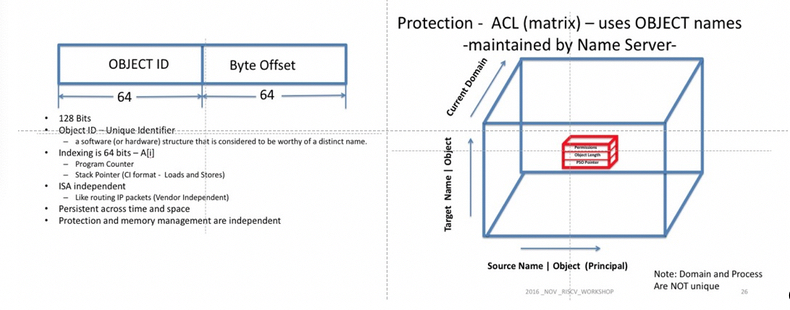
\includegraphics[scale = .5] 
{figures/figure1a.jpg}
\caption {128  BIT POINTER and ACL MATRIX  - FOUNDATION}
\end{figure}
\pagebreak
\subsection {SV128 Registers -  Protection and Address Translation}

Many registers are defined that facilitate the SV128 mechanisms.   These registers either contain SV128 addresses or integer values.  The SV128 domain protection model, is inherently non hierarchical in nature. Consequently many registers with the same name, exist in different domains. Thus, in general,  the notion of privileged registers (with some exceptions) DOES NOT exist.  Foe example,  lets define a register called:  STATUS, and the status exists, uniquely for each domain.  Executing the LOAD STATUS register,  only loads a value  into the STATUS register in the current domain.  This is a more salable approach, compared to historical mechanisms.




The registers currently defined are and their meaning:



\begin {itemize}
\item PC – Program Counter. This register contains the byte address of the currently executing instruction.
\item Current Domain  (CURRDOM)– This is a 2 bit register.  The value of this register is used to determine the current protection domain.
\item DCAT (DOMCALLTABLE) Domain Call Access Table - used for cross domain calls
\item DCAB (DOMCALLBASE) The base address of the Domain Call Access Table - One per  domain
\item ODTBASE (OBJECTDEFTABLE) –BASE OF Object Definition Table- Object\_ID indexes into table.  Process Wide
\item Object\_ID  base register (CURROBJECT)
\item Current PGAS node id (CURRPGAS).
\item RS1 – the RV128 integer register set.  128 bit wide.
\item HyperPresent – Is this a Hypervisor configured system

\end{itemize}





\pagebreak





%----------------------------------------------------------------------------------------
%	SECTION 3
%----------------------------------------------------------------------------------------
\section{SV128 Protection and Address Translation} 

This chapter specifies  the Protection and Address Translations mechanisms. When and where appropriate,  registers will be named.  At this time,  these registers are place holders. The objective of the described mechanisms is to support a hardware supported hypervisor implementation, and a limited domain based protection structure.  Additionally, a shadow stack mechanism is defined.  This permits the user to call an external library and constrain that library to  a well-defined data set as well as stack isolation.  

Additionally, in many cases,  definitions and tradeoffs follow or are heavily influenced by current Linux internal designs.   Linux running on SV128 is the target implementation. The purpose of this description is to establish the higher order mechanisms.  The actual registers and instructions follow. 

\subsection {Address Translation Overview}

Eventually more tables than currently show logical to physical translation (two sets) for an SV/128 bit virtual address, are provided.    For now, assume that this translation follows the RV64 RISC-V definitions for the 64 Object  (Byte) Offset.  Each Object Id,  indexes into a table   with the contents of this table entry denotes, among other things,  which RV64 address translation to be used.   In doing this,   it is much easier to support executable images for RV64 and RV32 binaries.  Also, Linux code will have been written that does all this for RV64.  Thus, only one more level of level of indirection is needed. It should be noted that the initial  indexing will more than likely be hashed.  This depends on how many Object Ids  are defined.

Since there are two sets of tables:  Hypervisor and No  Hypervisor.   There are two sections for logical to physical translation,  that deal with the presence or absence of a Hypervisor.

FORMAT OF LOGICAL ADDRESS SPACE

There are 2   logical address spaces that are supported on SV128 implementations.  The two are: RV64 (and RV32) for 64 bit RISC-V executable images. If these execute on a Hypervisor based system,  the page tables and protection structures need to adhere to the  structures defined for a 64 virtual address. The reason being that the kernel that is active is a 64 bit kernel and consequently creates 64  bit page tables. For native 64 bit address space applications,  the page tables and protection structures adhere to the structures defined by the SV128 architecture.



The format of a SV128 address space is:



\begin{figure}[h]
\begin{center}
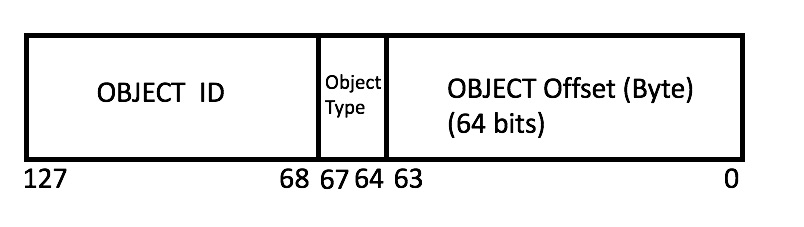
\includegraphics[scale = .4]
{figures/figure1b_objectid_image.jpg}
\caption{SV128 ADDRESS FORMAT}
\end{center}
\end{figure}


Even though 64 bits are allocated for the Object ID,  the first implementation will be restricted to 32 bits.  That  means that the logical address space of SV128 is 296  bytes.  This is  very similar to current Implementations of a 64 bit logical address space.  Most, if not, all current processor designs  only support 48 to 52 bits of the logical address space. The higher order 32 bits are reserved for future system use.

Indexing a SV128 logical address is mod 64.  This means ONLY the Object Offset takes part in the arithmetic indexing operation.  The OBJECT ID is NOT modified in any manner during indexing.

There are several values of the OBJECT ID that have predefined meanings.  As currently defined,  the Object Types defined are: 


\begin{itemize}
\item Object  Type= 0,1,2,3 -  Kernel Object.
\item   Object  Type = 4 – Byte offset is RV64
\item   Object  Type=  5 -  Byte offset is RV32
\item   Object   Type= 6 -   Interpret Object Bits 68 thru 95 (28 bits) as a PGAS Object
\item   Object Type = 7 -    Interpret Object Bits 68 thru 95 (28 bits) as a local OBJECT ID
\item   Object  Type = 8 thru 14 reserved
\item  Object  Type- 15 – Interpret Bits 68 thru 127 (60 bits) as an Object ID

\end{itemize}

The above encoding may eventually be HUFFMAN encoded.  This would eventually permit bigger OBJECT ID for certain objects.  I expect some form of IPv6 address will be defined.

Kernel Objects are statically defined to help create a hardware implementation that is secure against speculation from user space to kernel space.  An implementation may CHOOSE to disable speculation, no matter what form it takes,  when a Kernel Object is  being referenced.  When the protection system is operating  and references to  Object 0, 1, 2, or 3,  are permitted,  an implementation may choose to support hardware speculation.  An implementation may also choose to support or disable cross object speculation when In user space.

\subsection{Protection}

This chapter describes the protection structures  for SV128.  The protection structures are defined in a manner that directly supports the following RISC-V paradigm.



\begin{figure}[h]
\begin{center}
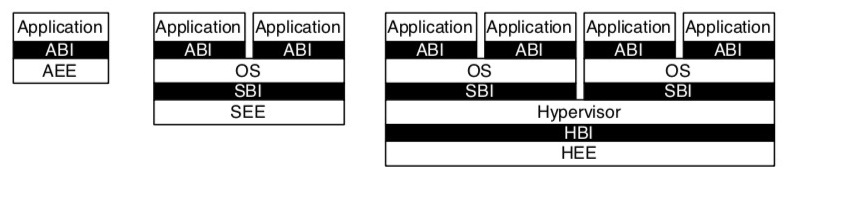
\includegraphics[scale = .4]
{figures/figure1c_riscv_stacks_privileged.jpg}
\caption{RISC\-V Privileged Stacks}
\end{center}
\end{figure}

\begin{figure}[h]
\begin{center}
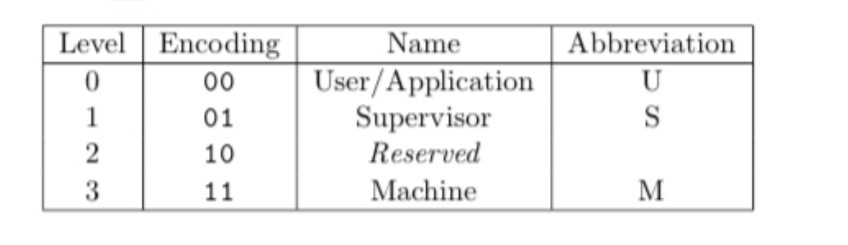
\includegraphics[scale = .4]
{figures/figure2_privileged_level_simple.jpg}  
\caption{RISC\-V PRIVILEGED LEVELS}
\end{center}
\end{figure}

Another way to depict this is  from the INTEL  VTx structures (see Figure~\ref{fig:intelvtx}).

However it should be noted,  that for SV128,  there is NO IMPLIED PRIVILEGED  LEVELS. there are 4 domains, equal in privilege.  To correctly manage system wide security polices,  there are 4 OBJECTS that are considered KERNEL  Objects.  Various capabilities can only  be performed by KERNEL Objects. Additionally for each domain a capability referred to as as SHADOW STACK is provided.  Thus permits users to incorporate external libraries in a hardware enforced SANDBOX  structure.  Consequently the RISC\_V privileged is now recast as follows:

\begin{figure}[h]
\begin{center}
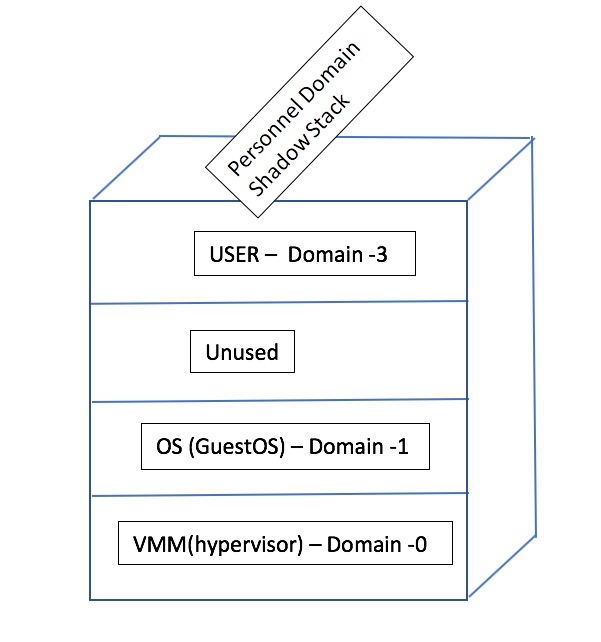
\includegraphics[scale = .4]
{figures/domain_levels_software.jpg}  
\caption{RISC\-V SV128 DOMAIN PRIVILEGED LEVELS}
\end{center}
\end{figure}


\begin{figure}[h]
\begin{center}
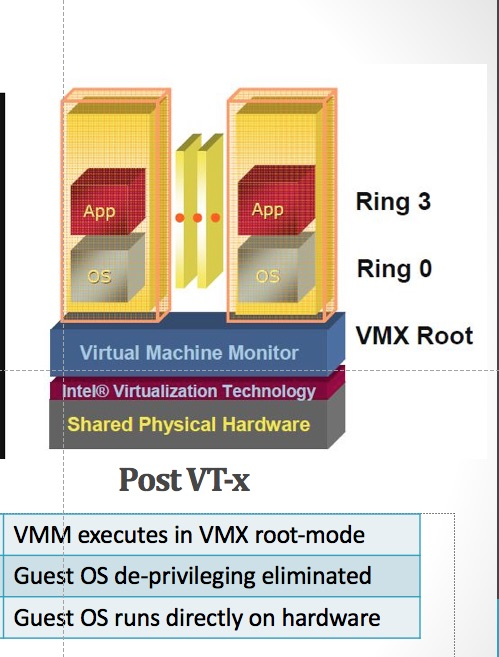
\includegraphics[scale=.4]{figures/figure2a_intelvtx.jpg}
\caption{Intel VTx structures\label{fig:intelvtx}}
\end{center}
\end{figure}


It should be noted,  that the static allocation of the OS to Ring 0,  by INTEL, precludes the direct incorporation of the address space and protection mechanism of Virtual Machine Monitor with the address space of the OS (noted as Rings 0 thru 3). This static allocation is appropriate for non-virtual machine monitor situations.  This is NOT the case for SV128. For SV128,  protection CONTEMPLATES a Virtual Machine Monitor.
\pagebreak
\pagebreak

\subsection{Domains}

The definition of SV128,  assumes from the onset,  the support of 4 non-hierarchical levels of privileged execution.  These 4 levels are:  USER/APPLICATION (Domain – 3).  SPARE,  OS (Domain -1), HYPERVISOR (Domain-0).   The definition of the protection structures is INDEPENDENT of the definition of the SV128 virtual address space.  When this virtual address space is visually examined,   as previously noted,  it is partitioned into OBJECT ID and OBJECT OFFSET. Some object enumerations may have static meanings and these meanings may have protection ramifications.  For an OBJECT ID equal all zero’s  (and other encodings) means the OS kernel object. The USER never references the Hypervisor Object. This helps  prevents various security breaches due to speculative execution. 

As will be noted the permissions of each of the 4 domains are independent of one another.  The 4 domains,  with hardware, directly supports  what is displayed in Figure 1. The objective of the creation and functioning of  these 4 domains,  is to directly support, in one homogeneous architecture, the software structures shown in Figure 1 and 2. When a memory reference is made,  access permissions as designated by the current domain are interpreted.  

While not currently implemented,  one can anticipate that over time,  the Hypervisor and OS kernel will become aware of each other.  SV128 anticipates this and consequently  defines its structures accordingly.

When the OS  or VMM is booted up,  a privileged register  (HYPER\_PRESENT) is set.  This register indicates the presence or absence of a Hypervisor.    The state of this register is used to determine logical to physical translation and other  VMM (virtual machine) operations. Various other registers are set when the VMM is booted.

Domains are defined to isolate and protect data from one part of the OS from user data.  One of the classical computer domains is RINGS.  They are hierarchical in nature.  Usually the user is in the ring that had the least privileges and the OS in the ring that had the most privileged.  Due to the hierarchical nature of rings,  various hardware implementations,  based on the definition of the logical address space exist.  Address references are mediated based on current   ring and target ring. This generally works quite will.  However, there are cases,  that the static inflexibility of this structure, leads to complex sharing structures.   Thus, for SV128 four non-hierarchical domains are defined. The OS may choose, via entries in the PTE to make data references hierarchical or not. Figure 5,  the format of a PTE shows the domain  permission fields in a PTE (4 bits).  When an address is translated from logical to physical the meaning and use of these fields will be specified.


\begin{center}
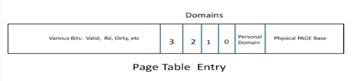
\includegraphics[scale = .9]
{figures/figure2b_pte.jpg}
\centering
\end{center}

\subsubsection{Domain Crossing}

Crossing a domain is mediated.  Arbitrary entry  points are NOT  permitted. When crossing a domain,  the domain call instruction sequence MUST access a table in the Called Domain. The base of this table is defined in a register called: DOMAIN\_CALL\_ACCESS\_BASE (DCAT). 


 Assume for description the DOMAIN call instruction has the following format:

\begin{figure}[h]
\begin{center}
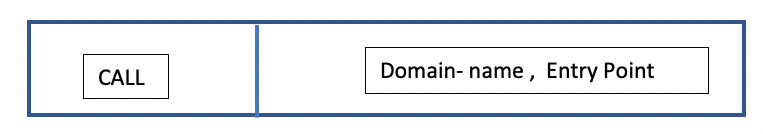
\includegraphics[scale=.4]
{figures/figure3_call_instruction.jpg}
\caption{Call instruction}
\end{center}
\end{figure}


\subsubsection{Domain Call Access Table}

When an OS is created, either due to either a native SV128 OS or a SV128 Hypervisor,  4 registers are loaded.  These 4 registers  contain the logical address of the Domain Call Access Table (DCAT),  one per domain.   These registers are:  Domain Call Access Base.  (DCAB). The structure of  these table is:

\begin{figure}[h]
\begin{center}
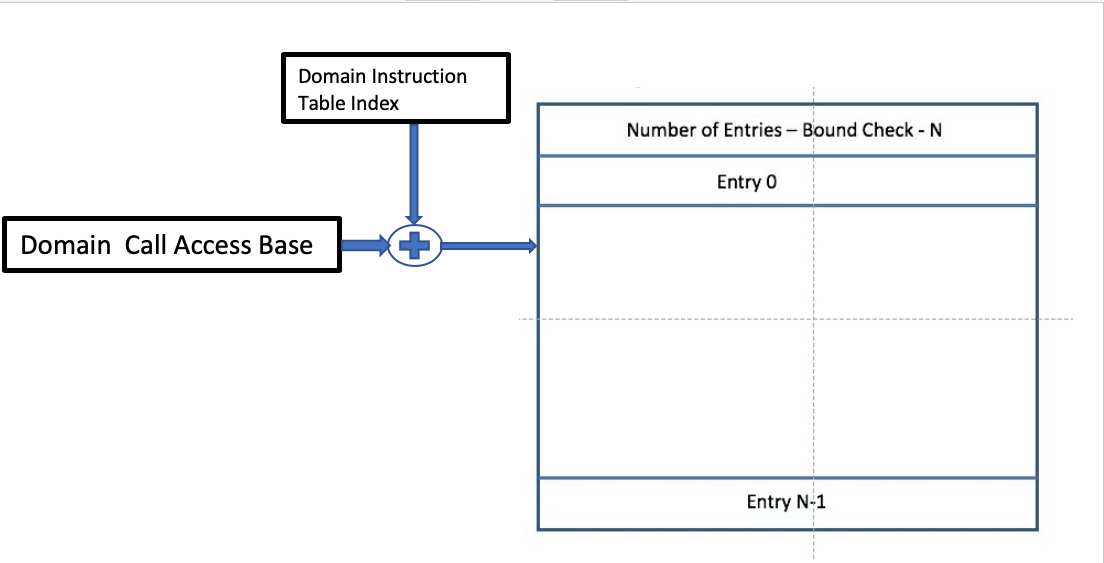
\includegraphics[scale = .4]
{figures/domain_call_table_index.jpg}
\caption{DOMAIN CALL ACCESS TABLE}
\end{center}
\end{figure}

		                 
		                 
The base of this table is referenced in the Domain Call  Access Base (DCAB) register. 


		                 
		                 
		                 
\subsubsection{Domain Call}		     
		                 
When domain call instruction is executed the following occurs.  The Domain Name specified in the Domain Call instruction  is used to logically reference the appropriate Domain Call Access Base Register (DCAB).

The first entry is used to perform a bounds check.  The entry point named  in the instruction (an integer - bits [15-0]) is compared to the Bounds Check  Value in  the DOMAIN CALL Access Table.  If  the specified entry point is valid,  then   the specified entry  point is used to index into the table and branch to the first location of the called routine.  There is NO OTHER WAY to transfer control from a caller to callee domain. The return domain instruction is the compliment of the CALL Domain. 

Additionally,  the  contents of the entry indexed,  128 bits has the following meanings.  

The lower 96 bits is the logical address of a valid entry point in the called domain,  becomes the new  value of the Program Counter (PC).  The higher order 5 bits are used for permissions and entry validity.  Bit 127 indicates that the table entry is valid (valid  =  “1”).  If not valid, a faults occurs. Bits [126-123]  indicate that a domain crossing from the current domain permitted.  Bit 126,  a “1” indicates that a call from domain 0 is permitted.  Bit 125 indicates that a call from domain 1 is permitted and so one. This structure is consistent with the non-hierarchical nature of domain.  This structure also permits certain entry points to be uniquely defined for particular routines for particular domains.



In addition to these transfer of control, a new stack is created  in the called domain.  The called domain may access the caller’s domain,  but the caller’s domain cannot access the called domain’s stack.


\textbf{It is the responsibility of the EACH domain to create its own DOMAIN CALL ACCESS TABLE.}

\subsubsection{Discussion of Object Definition  Table (ODT) Entry}

More  than likely the ODT entry will have 256 bits.  I would be appropriate for this unused entry to be a system wide Object Name when a hypervisor is present.  The current  64 bit Linux,  creates 64 bit unique process id's.  
Names that are uinqiue make it easier for the kernel (GuestOS or VMM) to manage resources. Creating this name, also  provides the ability to construct a system-wide TLB mechanism,.  Please see the section on TLB architecture.


\subsubsection{Domain Return}

In a non-hierarchical system the return is basically the same as the call. For SV128, the supporting structures are described in Figure 1, etc.  And this is hierarchical.  Thus, the RETURN from a domain call is:  switch stacks,  change the CURRDOM to the original caller’s domain.  Since the structures are hierarchical,  it can be  assumed that the PTE’s used by an inner domain,  have access to the caller’s domain data. 

For a detailed description of domain call and return, see Appendix A.

%----------------------------------------------------------------------------------------
%	SECTION 4
%----------------------------------------------------------------------------------------
\pagebreak
\section{Memory Translation}

\subsection{Translation of Logical to Physical Addresses}

There are two protocols for logical to  physical address translation.  One protocol is for the situation when there are only 3 domains used.  There is no Hypervisor or Virtual Machine.  The other protocol is for logical to  physical translation  when a Hypervisor or Virtual Machine is supported. The tables to translated logical to physical are straightforward in most cases.   This is especially true for the case of no Hypervisor.

When time permits,  the support for various   physical pages sizes will be specified.  Additionally, figures that show the various  page table levels will be provided.

\subsection{Translation With No Hypervisor: RV64}

The SV128 address space, though not necessarily protection, is hierarchical in nature. Figure 1.  (above) is a description of this.  Supporting this structure,  in hardware,  means that one needs to know the current address space and the  target space to be referenced. As part of the machine state (a register),  will be provided that denotes the current domain. For purposes of this description,  this 4 bit register is called: CURRDOM.   There are 4 domains.  Each domain is independent from one another.  There is NO implied hierarchical  ordering implied. (UNLIKE  RINGS).  Each domain has its own access bits (e.g., Rd, Wr, Exec, TBD). There are well defined calling and return protocols when a domain is called or returned.  Defining protection In this manner permits more extensible and opened protection mechanisms to be developed.  

The following is the  translation for RV64 of the current RISC-V ISA.  I am using this to describe what is appropriate for SV128.   The page table structure of the translation of a 48 bit virtual address for RV64 is:


\begin{figure}[h]
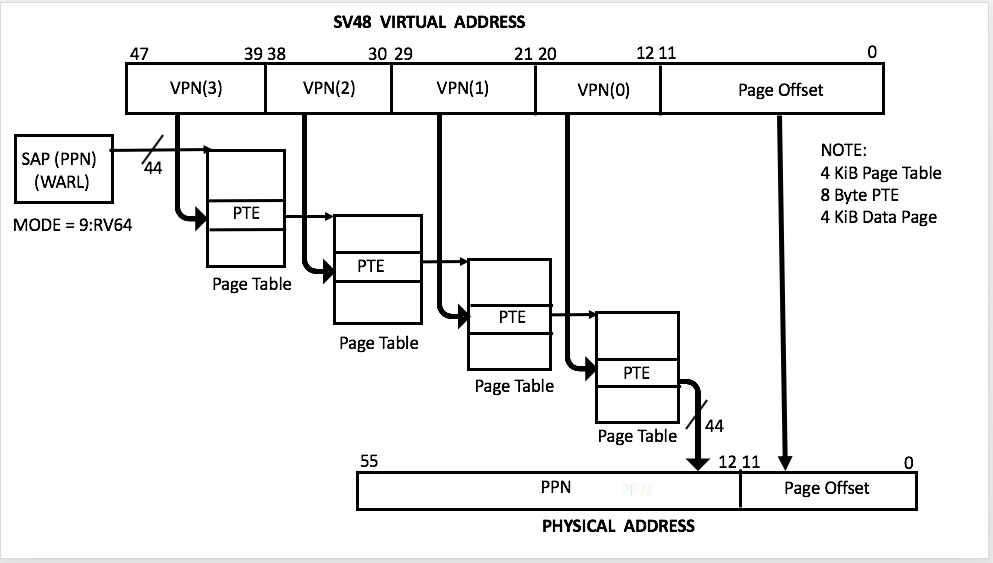
\includegraphics[scale=.4]{figures/figure4_sv48_translation.jpg}
\caption{CURRENT RISC-V TRANSLATION OF VIRTUAL TO PHYSICAL – SV48}
\end{figure}

\subsection{Translation With No Hypervisor: RV128}

For SV128 the address of the page table comes from an index (hash) of the Object ID of the  128 bit virtual address).  Thus, what is noted as SAP (PPN – WARL) for RV64 is replaced by this  hash. 

The hashed Object ID is used as an index into the OBJECT DEFINITION TABLE (ODT)).  The base of this table (on physical memory) is contained in the OBJECT Definition Table Base (ODTBASE). The Object Definition Table is Process Wide. The contents of a ODT entry and/or PTE contain permissions that control the access's an object has for a particular domain.

%               OBJECT_ID (HASHED)
         
\begin{figure}
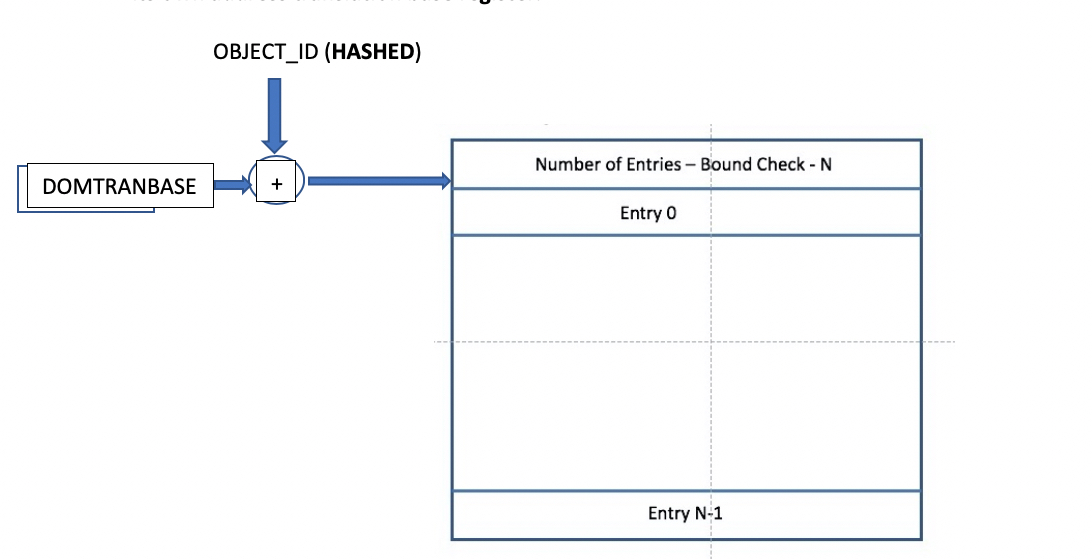
\includegraphics[scale=.4]{figures/figure4a_datt_translation_table.jpg}
\caption{INDEXING INTO OBJECT DEFINITION TABLE}
\end{figure}

The contents of a valid object indexed entry is as follows:

An entry can be Up to 3 64 bit words.  

The first word  contains 2 32\_bit fields.  The higher order 32 bits is a control field.   The bits in this field indicate:  the entry is valid or not and the type of  entry. The valid bit permits this table to be sparse.  The Object\_ID table is maintained by the OS or VMM.  When there is a VMM,  there is an Object Table per GuestOS instantiation.  The type of entries are:


\begin{itemize}
\item No bounds check on the referenced operand.  proceed with  accessing page tables for logical to physical translation.

A valid entry that points to an operand or structure.  A bounds check is needed to validate the reference is valid.  This is independent of the read, write, and execute permission bits. If there is a bounds check,  the third 64 bit word is used for the bounds check. If the bounds check succeeds,  the  logical to physical translation is executed. The domain permission bits in the higher order 32 bits are used to determine if the reference is valid (using the CURRDOM register).

\item Bounds check on the referenced operand (using the 64\_bit byte offset of the operand reference)

A   valid entry that  indicates that word 2, contains the physical address of the page tables required for logical  to physical address translation.

A field in the higher order 32 bits indicates that the type of   translation required for operand accesses to the referenced Object\_ID. These fields are  consistent with the current definitions of the RISC-V  RV64 and RV32,

\end{itemize}
The lower order 32 bits of the first 64 bit word is reserved.  It is anticipated that if the Object\_ID lookup is a hashed lookup;  this field will contain the 32 bit name of the Object.  This is required for contemporary  hashing algorithm.  One needs to know if the hashed  index , in fact, accesses the correct Object\_ID table entry

As an aside,  the contents of the Object\_ID table entry can be viewed, if one wants, as a CAPABILITY.  For this situation,  there is no need to tag or partition memory in a way, that prevents forged capabilities.

\subsection{Discussion - ODT Format and Contents}
\label{Discussion - ODT Format and Contents}

If the ODT entry were expanded to 256 bits,  then the entries should be:

\begin{itemize}

\item word 1  - control,  page table configuration,  and permissions.  ObjectId for Hash Table assistance.
\item word 2 - physical address of first level page table
\item word 3 - bounds check  on 64 bt byte offset 
\item word 4 - system wide virtual address,  created by Hypervisor when present
\end{itemize}

The reason for the inclusion of word 4,  system wide wide virtual address, to:  be consistent with the current 64 bit Linux conventions for managing resources by the kernel and to provide a mechanism for a Persistent State TLB. Please see the section on TLB Discussion for more details.  The following is a diagram of the current Linux kernel system wide naming.  How would this be extended,  for SV128?

Word  4   has  meaning if a TLB with a persistent architecture is implemented.  This means process multiplexing DOES NOT  flush the TLB.  This can have meaningful imnpact on performance.  There maybe several   definition of word 4.  Thus,  for now, assume in word 1,  there is a 3 bit field that determines how the hardware will use word 4.  When there is a selected value in word 4,  the TLB will associate this value,  the indexed Object\_ID  and the Byte Offset for lookup purposes.

The encodings are: 

\begin{itemize}
    \item 000 - Do NOT USE
    \item 001 - use the lower order 32 bits
    \item 010 - use the higher order 32 bits
    \item 011 - use the entire 64 bits
\end{itemize}




\begin{figure}[h]
\begin{center}
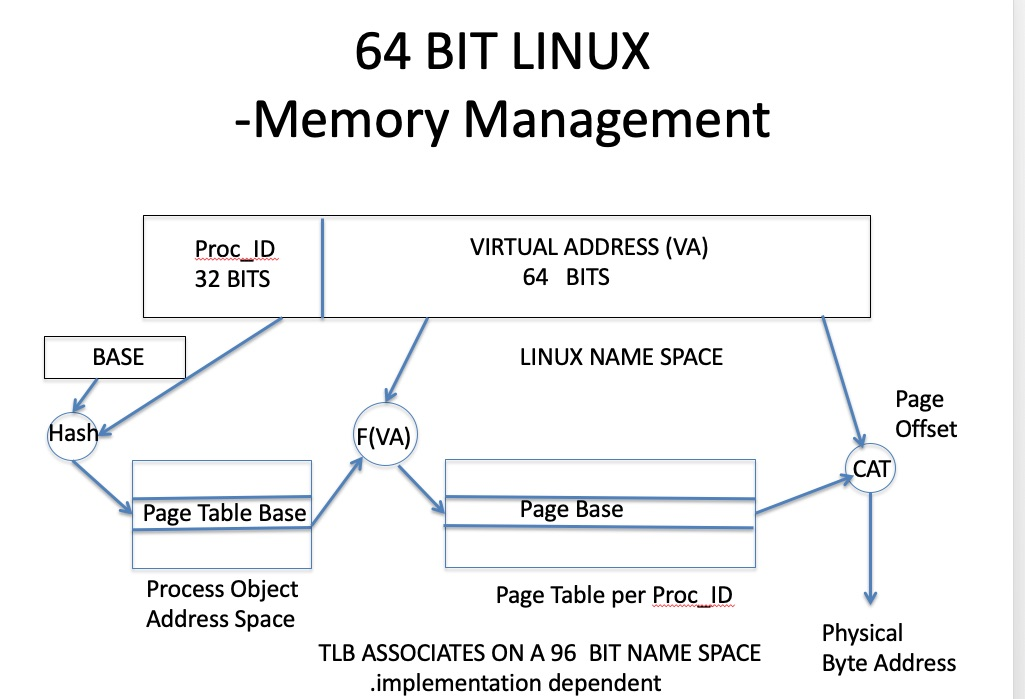
\includegraphics[scale=.3]{figures/96_bit_linux.jpg}
\caption{CURRENT 64 Bit Linux Kernel structures}
\end{center}
\end{figure}

\pagebreak

\subsection{Page Table Entry - Fields}

The Format of a PTE (denoted as VPN (0) is the above figure) is:

\begin{figure}[h]
\begin{center}
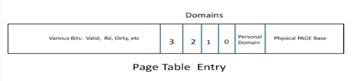
\includegraphics[scale=.8]{figures/figure2b_pte.jpg}
\caption{PAGE TABLE ENTRY}
\end{center}
\end{figure}

Each of the above domain fields is 4 bits wide.  These 4 bit indicate permissions (or lack thereof) for READ,  WRITE,  EXECUTE,  TBD. (perhaps reduce to 3 later on). One possibility for the unused bit to trap to a routine that mediates the access in some controlled  manner (like time of day)

\begin{figure}[h]\begin{center}

\includegraphics[scale=.4]
{figures/figure5a_domain_permissions.jpg}
\caption{PTE PERMISSION}
\centering
\end{center}
\end{figure}

Assume the LOAD instruction is executed.  The load instruction generates a SV128 virtual address.  This virtual address needs to be translated to a physical address.  Only for purposes of this description, assume that we have translated the virtual address and now have accessed the final PTE needed to reference the desired operand (data or procedure), as shown in Figure 5 Page table Entry.   The following now occurs.  The value in the CURRDOM register is compared to the corresponding domain field of this PTE.   If a read is requested the read permission bit is examined.  If a read is authorized,  the referenced operand is fetched.  If a write is requested,  the write permission bit is examined.  If a write is authorized the referenced operand is written.  If a transfer of control is requested,  the execute permission bit is examined.  If  a transfer is authorized,  a transfer of control happens.  The CURRDOM is not  CHANGED.

The domain access permission bits for intermediate page table entries are NOT interpreted.   Only for the final PTE permission bits that references the operand  are interpreted.

%----------------------------------------------------------------------------------------
%	SECTION 5
%----------------------------------------------------------------------------------------
\pagebreak
\section{Shadow Stack}


\begin{figure}[h]
\begin{center}
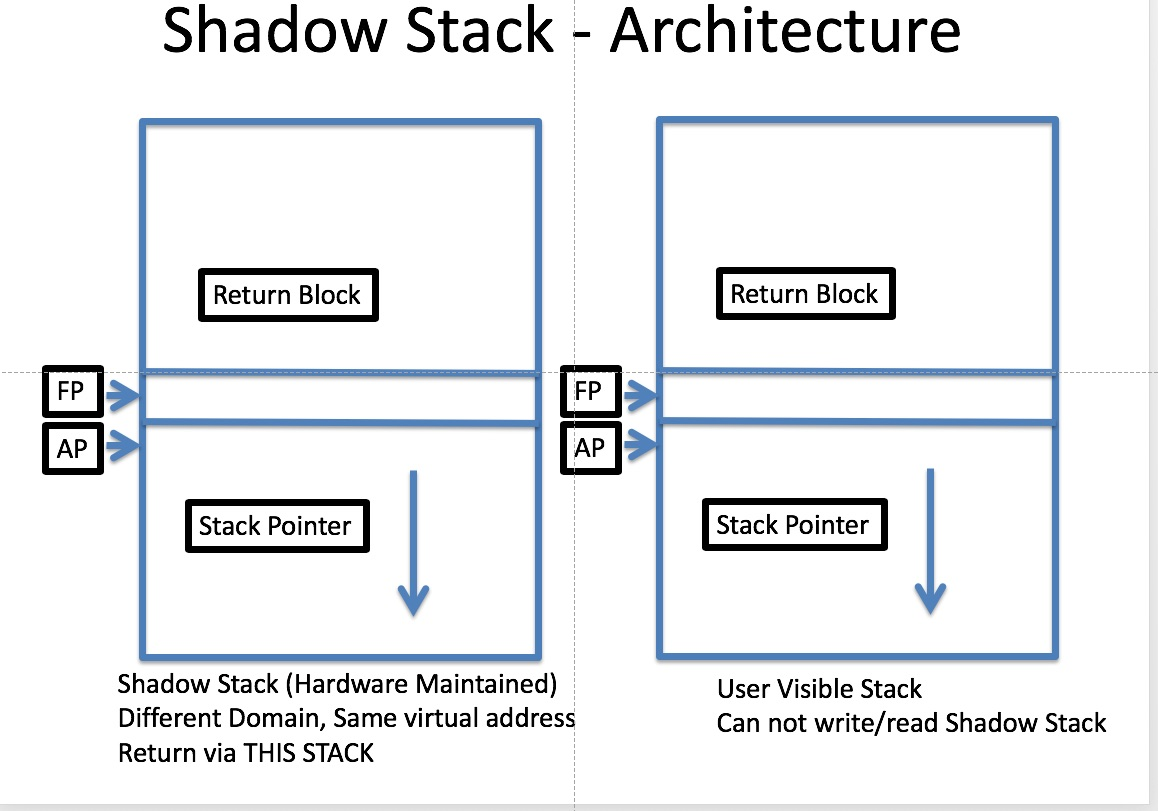
\includegraphics[scale = .4]
{figures/figure6_shadow_stack.jpg}
\caption{SHADOW STACK  ARCHITECTURE}
\end{center}
\end{figure}


PARAPHASING  a phase from Greek Mythology: Beware of GEEKS bearing gifts.

Protection comes in many forms.  The most dominant form is protection of  the OS Kernel/VMM from user access. This is generally supported via the definition of instructions that  can only be executed by the Operating System.  This assists in separating user data and control from OS  data and control.  In contemporary protection systems one would also like to provide a similar level to the USER.  this is the case, when the USER calls an externally provided software routine,  a library call. In a manner similar to the OS/USER structure, SV128 provided a level of library isolation and control via the creation of a SHADOW STACK  and with mediated operand access by the library to the caller's data (SANDBOX).

The characteristics of the shadow stack are:  A separate set of subroutine control registers (SP and FP),  and an additional domain field in the PTE.  In essence a PERSONAL DOMAIN, for the user is defined and hardware  This functions is as follows.

The user executes the subroutine call instruction.  When the address of the called routine is translated (using defined entry points as in a domain call), using the Domain Translation Base register of the CURRENT DOMAIN)  the PERSONAL DOMAIN bits of the final PTE are interpreted. If the appropriate bit is set,     a shadow stack call is initiated. This results in a new set of stack management registers.  The callers stack management registers are NOT  accessible to the called routine.

This also now means,  that the  address translation of the memory references from the called routine  NOW INTERPRET  the personal domain bits of the PTE.  (The translation space is still the caller’s space).Thus, no new PTE translation tables are required.   In this manner, the USER (the caller) can indicate that its data structure is only read only or no access (SANDBOXING on a page basis).  When the called routine exits from the call (a return),  the caller stack management registers are used.  Thus, the called routine, with these hardware enforced features,   is restricted to particular caller defined data references and return control This is similar to the mechanisms provided to protect and mediate the interactions between and OS kernel/VMM.  But now extended,  in a limited manner to the USER.




For example,  assume the user has 1 GByte of data managed by a RV64 address space for one object.   The page tables indicate the physical location and permission bits for this 1 GByte of data.  The user calls a library that it wishes to be SANDBOXED and permission to only read one particular 4 KBytes of data.   Prior to the call,  the user makes a sys\_call.  The sys\_call results in an entry point for the called routine being created in the Domain Address Translation Table.  Additionally, the PTE for the referenced page is marked for the appropriate permissions in the PERSONAL DOMAIN field. All other permission bits are disabled.  Thus, the called routine can only read/write the specified 4 KByte page,  even though the library is in the same domain and uses the same page tables.






%----------------------------------------------------------------------------------------
%	SECTION 6
%----------------------------------------------------------------------------------------
\section{Logical to Physical Address Translation with a Hypervisor}


This is, perhaps the most difficult   protocol to support in hardware.  The reason is simple,  the OS thinks it manages ALL of physical memory.  But there  are multiple OS’s.  Thus, if this was allowed in some uncontrolled manner, there would be conflicts for physical memory allocation. In many cases,  additional registers are defined.  These registers, in many cases,  directly support VMM.  The objective for SV128 is minimizing the overhead of VMM which results in minimum performance degradation relative to non-vmm systems.

\subsection{Problem Statement}

The GuestOS in Figure~\ref{fig:guest-logical-physical} creates the page tables for its users.  The GuestOS assumes it has TOTAL control of the physical memory actually implemented (as it would normally have).  Thus, is allocates physical memory and  consequently fills in PTE’s for a user process accordingly.    To make this work, with multiple OS’s,  the VMM needs to allocate subsets of physical memory to each running OS.  For example,  assume there is 32 GBytes of physical memory.  Also, there are 4 executing GuestOS’s.  The Hypervisor could allocate physical memory as follows (ignoring overheads).  16 GByte to GuestOS \#1.  8 GByte to GuestOS\#2,  and 4 GByte to GuestOS\#3 and OS\#4. Thus the 32 GBytes pf physical memory is allocated.  

There are several consequences of the above.  Each GuestOS has to know how much physical memory it is allocated.  Let’s assume this is in a register called:  OS\_PHYS\_MEMORY (OSPHYMEM).   Only the OS and VMM can modify this register.  However, when each GuestOS creates page tables for its users,  it assumes that physical memory starts form ZERO.  You cannot, in this example,  have each OS allocating pages from physical address ZERO. Thus, the physical address’s in each GuestOS page tables  somehow have to be redirected or not used. So how do we do this? One way is to always redirect physical address when a VMM is present.  That works but adds incredible about of overhead for logical to physical translation.  In essence each translation step requires 2 steps.  Another  method,   called a SHADOW or NESTING approach is what will be supported.  There are several mechanisms that need to be defined for this to work.

Using the translation of RV32 the following is defined. (for describing only)

\begin{figure}
\begin{center}
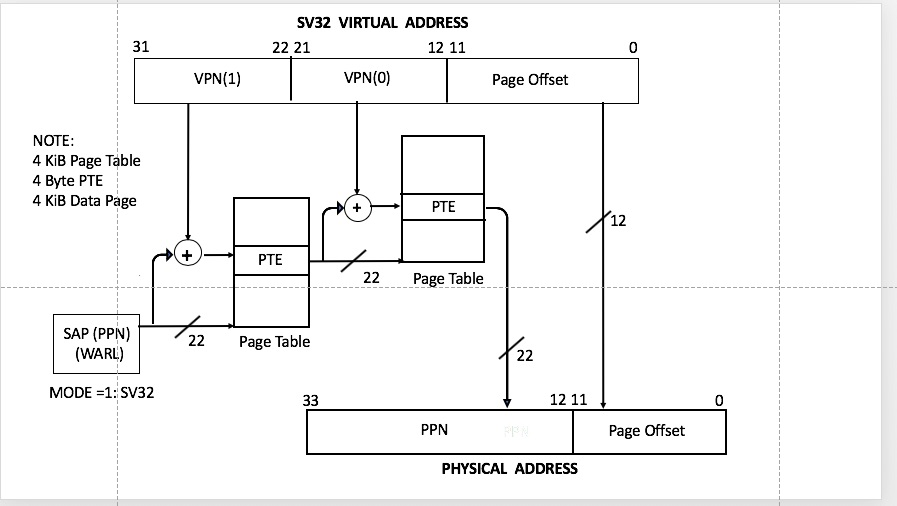
\includegraphics[scale = .4]
{figures/figure7_rv32_pte.jpg}
\caption{GuestOS created page tables for translating logical to  physical (OS Physical Address Space)\label{fig:guest-logical-physical}}
\end{center}
\end{figure}


The VMM creates the following


\begin{figure}
\begin{center}
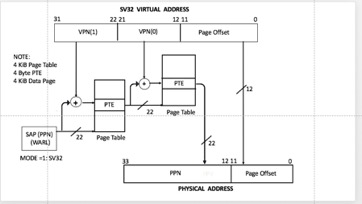
\includegraphics[scale = .9]
{figures/figure8_hypervisor_page_table.jpg}
\caption{Hypervisor  page tables for translating logical to physical (VMM Physical Address Space)}
\label{fig:hypervisor pagetables}
\end{center}
\end{figure}

There is a VMM status  control register.  When VMM is enabled this results is the following: The base register for address translation for RV32 is changed from SAP (PPM WARL)  to the VMM\_REG. 

 In reality, as a result of a physical address base for each Object\_Id,the VMM\_REG becomes the    This register,  the Object Definition Base Register (ODTBASE)  can only be changed when the current domain is 0, when a Hypervisor is present.


 The Hypervisor created page tables, in the VMM address space are NOW used (see figure ~\ref{fig:hypervisor pagetables}), in place of the GuestOS created page tables for logical to physical  translation.   In essence the overhead for a VMM logical to physical  translation is substantially reduced.   The indirection previously described is reduced to ONE indirection, once upon   initiation of lookup,  rather than for all physical memory references external to the VMM. This approach is NOT NEW and has been implemented in several systems.

In essence the GuestOS created page tables are made redundant.  When these tables are initially created by the GuestOS,   the instructions used are trapped to the VMM.  We need to define what privileged instructions are executable in domain 1 and domain 0.  (thus, one benefit of the domain protection system). In this way,  the Hypervisor knows what the GuestOS is doing, but in allocates REAL physical pages.  The GuestOS allocation of physical pages is  meaningless with respect to real physical memory addresses. Thus, the PTE’s created by the Hypervisor are IDENTICAL to the PTE’s created by the OS, OTHER than physical address’s.  

We need to consider at least one more item.  The user requests more memory from the GuestOS, during the running of the application. ( MALLOC).  For normal GuestOS running,  once memory is allocated or deallocated the appropriate PTE’s are modified (indicating valid PTE for new data, or invalid PTE for deallocated date). How do we do this, in the case of VMM and the OS page tables are meaningless?   How do we make changes in a PTE when an application is running?

The following works for this situation.  Assume we need to modify the PTE’s of VPN(1) and VPN(0) of the logical address space  to correctly execute the allocation or de-allocation of physical memory. We need to know one more item.  When the GuestOS is booted for the first time,  it establishes a correspondence  between virtual and physical memory. (Figure 9 and 10). This correspondence is as follows.  If there is 32 GBytes of physical memory,  the first 32 GBytes of Virtual Address Space of the Hypervisor is statically allocated  to this virtual to physical  mapping. Meaning when the VMM runs in virtual addressing mode,  it addresses ITS OWN memory mapping as virtual equals physical.  The same mapping is done for the GuestOS in domain 1.  But in this case, only for the physical memory allocated by the Hypervisor. (For Example, OS\#1 – 16 GBytes out of a possible 32 GBytes).

This means that a GuestOS (not VMM) physical address is actually a mapped virtual address spanning the physical memory allocated to the OS by the Hypervisor.  Thus, if we know when the GuestOS is referencing this memory,  we can redirect the translation  to the Hypervisor  to the real physical address or in this case, a PTE (Remember a PTE is always physical addressed.  Something have to be real).  

How do we do this?  We know the physical memory allocated to the GuestOS by the Hypervisor.  Let’s call this PHYSICAL MEMORY.   Under normal operation,  any user virtual address uses the Hypervisor created page tables.  So, we need to know when the GuestOS  references what it believes to be physical memory.   This is  accomplished in the following manner. 

As previously described,  the GuestOS kernel references the page table using a virtual address.  As with a user vertical address,  this GuestOS kernel virtual address is translated using the page table in the Hypervisor address space (Kernel 0).  When these page tables are created ALL the PTE’s are labeled READ ONLY.  Thus, any attempt to modify the contents of a user page table (in the VMM space),  by the GuestOS is trapped.  This trap is vectored into the Hypervisor space.

The consequence of all this results is the following.  Any and all GuestOS (Domain 1) actions that access and/or modify the PTE’s of the processes it manages are redirected to the PTE’s maintained by the Hypervisor in Domain 0.  There is no loss in performance during the normal execution of an application.

The following figures are used to explain this mapping of physical to virtual for the kernel.

\begin{figure}
\begin{center}
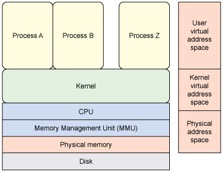
\includegraphics [scale = .5]
{figures/figure9mapping_logical_physical.jpg}
\caption{MAPPING OF PHYSICAL TO LOGICAL ADDRESS SPACE}
\end{center}
\end{figure}



\begin{figure}
\begin{center}
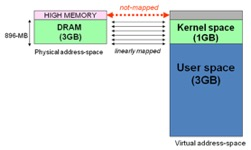
\includegraphics[scale = .5]
{figures/figure10_kernel_physical.jpg}
\caption{VIRTUAL ADDRESS SPACE AND KERNEL PHYSICAL ADDRESS SPACE}
\end{center}
\end{figure}


%----------------------------------------------------------------------------------------
%	SECTION 7
%----------------------------------------------------------------------------------------
\section{TLB Architecture and Discussion}

While  various approaches can be discussed and described,  there is one TLB characteristic that is the most important,  the working set size managed.   Thus, if there is a 32 GBytes of physical memory,  the working set of the TLB must be at least 32 GBytes.  This has to be true even for small page sizes.

The next feature always discussed is the associative approach.  Meaning does the TLB have to be purged after each process switch or not?   If not purged how is some level of global uniqueness maintained.  For SV128,  knowing that virtual address are created from domains, provides one type of uniqueness.    For the first implementations,   the use of the Linux Unique PID (32 bits) may be a good and rational choice.  This would be true if we choose a NON purge strategy when we have process multiplexing.

Before a description of 3 possible TLB architectures,  the following is how Linux views the virtual address of current 64-bit virtual address architectures.

\begin{figure}
\begin{center}
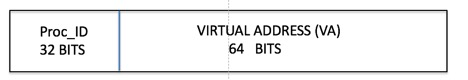
\includegraphics[scale = .7]{figures/figure11_linux_kernel_address.jpg}
\caption{VIRTUAL ADDRESS SPACE MANAGED BY THE 64 BIT LINUX KERNEL}
\end{center}
\end{figure}


Linux maintains up to 2  exp (32)  process  id encodings. 
Linux attempts to assign a global unique name.  Linux manages this table for name allocation,  name  revocation, etc.  

The possible TLB architectures are:

One implementation is to associate only a 64 bit virtual address.  This means the TLB only has the working set of ONE PROCESS.  Thus, upon process multiplexing,  the TLB must be purged.  This is the simplest  implementation.

The second  implementation is to associate on the 96 bit kernel managed virtual address.  Thus, upon  process multiplexing  there is no need to purge the TLB.  The tradeoff is higher performance and lower TLB page walking when multiple processes are switching.


The third implementation is only relevant when a VMM is present.  As noted before the Linux  created and managed 96 virtual address is  unique for  the case where there is only one Linux kernel.   When there is a VMM,  this is not the case.  So how can, if we want, create a TLB that DOES NOT have to be purged when there is multiplexing among Linux kernels?  This can be done by appending the PHYSICAL address of the page tables created by the Hypervisor for each instance of a Linux kernel.  By definition the physical address of the page tables for each Linux kernel base to be unique.  Define this entity (in a register) 	PHYSICAL KERNEL BASE (assume 40 bits). This is the register noted as VMM BASE in Figures 7 and 8.    Thus if one wants to create a TLB that is unique for ALL instantiations of all Linux kernels,  the virtual address that is associated has the following structure. 

Please the section,
\ref{Discussion -  ODT Format and Contents}  for how the definition of an Object\_ID  can be used by the TLB.


\begin{figure}
\begin{center}
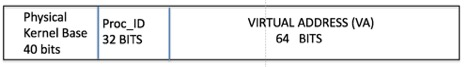
\includegraphics [scale = .7]
{figures/figure12_address_tlb_lookup.jpg}
\caption{Address used for TLB Lookup}
\end{center}
\end{figure}

%----------------------------------------------------------------------------------------
%	SECTION 8
%----------------------------------------------------------------------------------------
\section{ISA and Traps/Faults}

The stardard risc-v isa is supported in SV128.  The  general registers are extended to 128 bits. There will be several instructions defined that deal with domain crossing.  Instructions that load and store the various previleged resgiters will also  need to be defined.  Once there is agreement on the logical address and  protection mechanisms,  these instructions will be defined.

There are two possible approaches to the handling of traps, daults,  and interrupts.  One approach is to extended the RV64 definiton to  accomodate 128 bit pointers.  The other approach is to define a  different paradigm.











%----------------------------------------------------------------------------------------
%	SECTION 9
%----------------------------------------------------------------------------------------
\clearpage
\section{SV128 Machine Organization}
\label{sec:SV128MachineOrganization}

\subsection{SV128 Extension ISA Requirements}

The SV128 instruction set extension described herein is classified 
as a \textit{brownfield} extension with respect to the core RISC-V 
machine state.  In this manner, fits within the existing RISC-V instruction 
formats and encodings.  However, the SV128 extension does instantiate 
additional machine state in terms of user-visible and supervisor registers.

The SV128 specification functions an extension to the existing RV64I~\cite{RVSpec} 
base instruction set specification (and all inherited instructions therein).  In this 
manner, the SV128 extension is truly an extension, rather than a full expansion 
of the register \textit{XLEN} and the associated ALU.

\subsection{SV128 Implementation Requirements}

The goal of this specification is to outline the required encoding, register extensions 
and associated supervisor level functionality required to implement the SV128 
RISC-V extension.  It does not, however, imply any specific required implementation 
functionality unless otherwise noted herein.  Specific topics that are deliberately 
left up to the implementor can be summarized as follows:

\begin{itemize}
\item \textbf{Caching}: This specification does not require or prohibit the use of data caching 
when operating with 128-bit addressing.  It is up to the implementor to define if/how data caching 
is present and/or utilized.  

\item \textbf{Address Encoding}: This specification does not define any specific 64-bit or 128-bit 
address encoding format beyond what is described in the base RV64I specification.  Implementors 
may choose to utilize a partitioned addressing schema, a flat schema or combinations thereof.    

\item \textbf{Scalability}: This specification does not define the scalability of the least significant 
or most significant 64-bit address words.  For example, it is well within the implementor's power to 
utilize a 48-bit base address encoding and a small number of most significant (extended) encoding bits.

\item \textbf{Extended Memory Translation}: This specification does not require the use of any 
specific paging and/or virtual to physical translation methodology.  It is up to the implementor to define 
if/how virtualized memory access is implemented for the extended addressing.

\item \textbf{Memory Controllers}: This specification does not mention, nor require any specific 
location or implementation of the memory controller (et al. downstream memory components).  It is 
up to the implementor to define how/where the memory controller is implemented based upon the 
target system architecture requirements.

\item \textbf{Memory Bus/Interconnection}: This specification does not mention, nor require any 
specific memory bus or memory interconnection infrastructure.  It is up to the implementor to define 
how the memory units are connected to the target memory device or devices.

\item \textbf{Pipeline Model}: This specification does not mention, nor require any specific 
core pipeline model.  It is up to the implementor to define how the SV128 instructions are 
implemented.

\item \textbf{Virtualization}: This specification makes no mention of implementing a virtualization 
layer on top of SV128-style addressing.  Do not expect that SV128 addressing modes will 
automatically function with pre-defined RV64I virtualization mechanisms.  This is beyond the 
scope of this document.

\item \textbf{Enclaves}: This specification makes no mention of implementingSV128 functionality 
associated with system or machine-level security enclaves.  Any security-related functionality 
required to enforce enclaves on a system with SV128 extensions is beyond the scope 
of this document.

\end{itemize}

\subsection{SV128 Supervisor Specification Requirements}

\subsubsection{Machine ISA Register {\tt misa}}

As noted by the supervisor specification~\cite{RVSuperSpec}, the 
\textit{misa} CSR register is an XLEN-bit \warl\ read-write register reporting 
the supported ISA by the hart.  Normally, the MXL (Machine XLEN) field 
encodes the native base integer width as shown in the supervisor specification.  
In the case of SV128, this value is set to represent a 64-bit base ISA (\textit{MXL=2}).  We do 
not override this value as the SV128 implementation described herein does not 
natively modify the register width of the general purpose registers beyond 64-bits.    

\begin{figure*}[h!]
{\footnotesize
\begin{center}
\begin{tabular}{c@{}c@{}J}
\instbitrange{XLEN-1}{XLEN-2} &
\instbitrange{XLEN-3}{26} &
\instbitrange{25}{0} \\
\hline
\multicolumn{1}{|c|}{MXL[1:0] (\warl)} &
\multicolumn{1}{c|}{\wiri} &
\multicolumn{1}{c|}{Extensions[25:0] (\warl)} \\
\hline
2 & XLEN-28 & 26 \\
\end{tabular}
\end{center}
}
\vspace{-0.1in}
\caption{Machine ISA register ({\tt misa}).}
\label{misareg}
\end{figure*}

As stated in the supervisor specification, the \textbf{Extensions} field encodes the presence of the 
standard extensions via a single bit per letter of the alphabet.  Per this notional encoding, 
the ``I'' bit (bit-8) must be set for all implementations that support SV128.  Further, we also dictate 
that the ``X'' bit (bit-23) must be set to indicate a non-standard extension.

\begin{commentary}
Given that SV128 is currently a non-standard extension, the ``X'' bit must be set.  However, 
portions of this specification may be integrated into the official SV128 specification 
that will become an officially supported extension.
\end{commentary}

\subsubsection{Supervisor Cause Register ({\tt scause})}

Per the supervisor specification, the {\tt scause} register is an XLEN-bit read-write register 
formatted as per Figure~\ref{scausereg}.  The SV128 specification does not add any specific 
Exception Code values to be placed in the \wlrl\ field.  However, much in the manner of 
normal load and store operations from RV32I and RV64I, the SV128 extension has the ability 
trigger the codes listed in Table~\ref{scauses}.   

\begin{figure*}[h!]
{\footnotesize
\begin{center}
\begin{tabular}{c@{}U}
\instbit{XLEN-1} &
\instbitrange{XLEN-2}{0} \\
\hline
\multicolumn{1}{|c|}{Interrupt} &
\multicolumn{1}{c|}{Exception Code (\wlrl)} \\
\hline
1 & XLEN-1 \\
\end{tabular}
\end{center}
}
\vspace{-0.1in}
\caption{Supervisor Cause register {\tt scause}.}
\label{scausereg}
\end{figure*}

\begin{table*}[h!]
\begin{center}
\begin{tabular}{|r|r|l|l|}

  \hline
  Interrupt & Exception Code  & Description \\
  \hline	 
  0         & 2               & Illegal instruction \\   
  0         & 3               & Breakpoint \\
  0         & 5               & Load access fault \\
  0         & 7               & Store/AMO access fault \\
  0         & 13              & Load page fault \\
  0         & 15              & Store/AMO page fault \\
  \hline
\end{tabular}
\end{center}
\caption{SV128 Supervisor cause register ({\tt scause}) values after trap.}
\label{scauses}
\end{table*}

\subsection{SV128 Extended Addressing Logic}

At the core of the SV128 implementation is the ability to utilize existing RV64I 
binary blobs without issue.  In this manner, the SV128 extension makes use 
of the base RV64I register length, memory operations and ALU functionality.  
They key portions of the SV128 functionality and associated address mode 
is implemented via an extended register file that is mapped to a series 
of base registers as well as a set of SV128-specific instructions to perform 
standard load, store and register manipulation of extended 128-bit addresses.  We 
see this extended register set depicted in Figure~\ref{fig:machineorganization}.  

\begin{figure}[h!]
\begin{center}
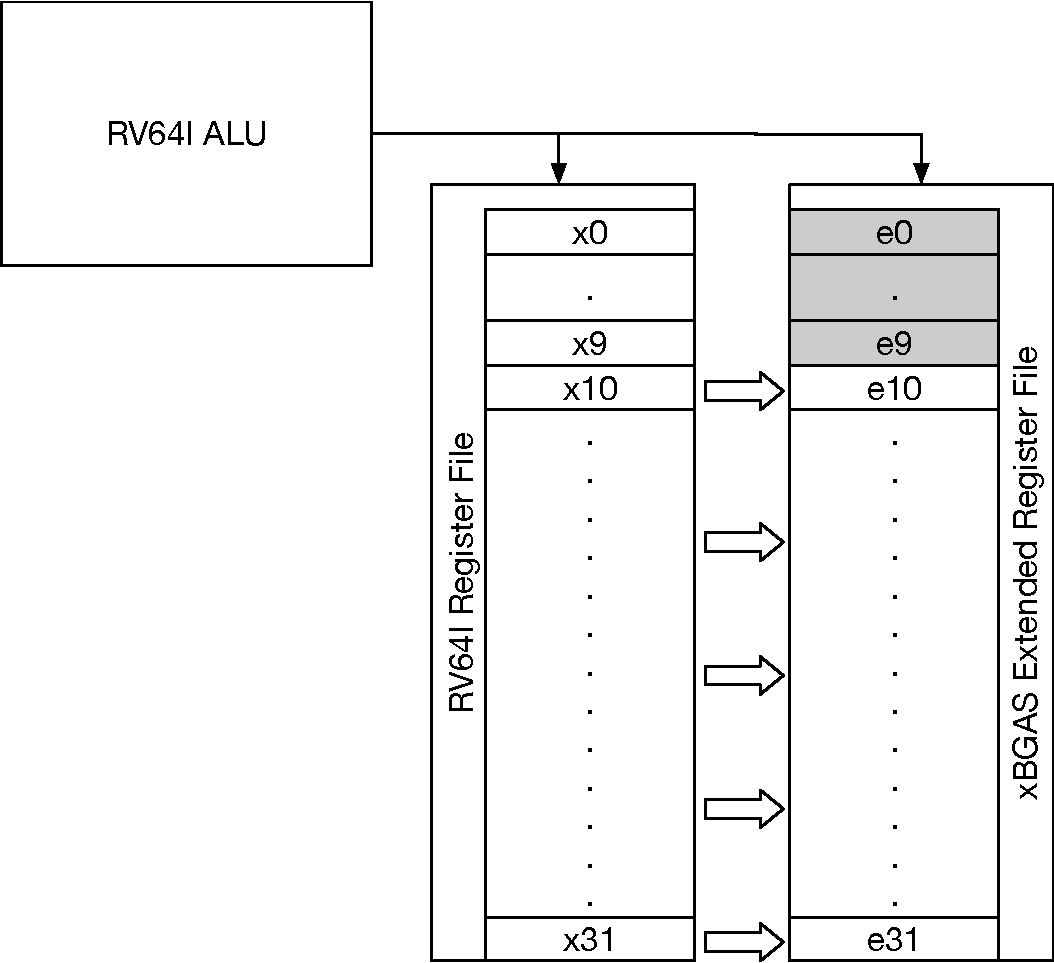
\includegraphics[width=3in]{figures/rv128imachorg.pdf}
\caption{SV128 Machine Organization}
\label{fig:machineorganization}
\end{center}
\end{figure}

In the aforementioned figure, note the specific mapping of base registers 
(\textit{xN}) to extended registers(\textit{eN}).  For each of the base 
registers beginning at index \textit{0}, we map a complementary extended 
register at the same index.  In this manner, SV128 memory operations 
utilize both the base and extended registers at the target index in the process 
of formulating the extended addressing schema.  However, also note that 
the first ten indices (\textit{0-9}) cannot be utilized for addressing.  These 
indices are reserved for operations in the memory translation layer.  This is 
analogous to the first ten indices in the general purpose register file 
that are specifically allocated to various operations associated with instruction 
handling (\textit{sp}), frame handling (\textit{fp}), context save/restore 
and hard encoding (\textit{zero/x0}).  As a result, these registers cannot be 
utilized in generating extended addresses for SV128 memory operations.  
Any attempt to utilize extended registers below index \textit{10} will 
result in an exception.    

\begin{figure}[h!]
\begin{center}
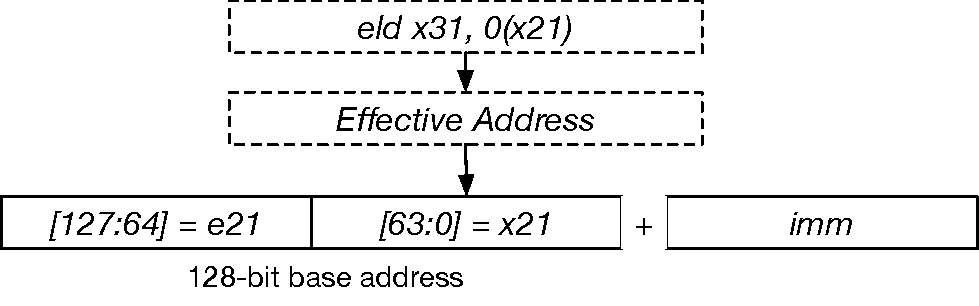
\includegraphics[width=3in]{figures/effectiveaddress.pdf}
\caption{SV128 Effective Address Calculation}
\label{fig:effectiveaddr}
\end{center}
\end{figure}

Given the aforementioned machine organization, we may also describe the SV128 addressing methodology.  
Figure~\ref{fig:effectiveaddr} depicts how SV128 load and store operations generate effective addresses.  For each 
given SV128 memory operation, we see that the base register index encoded in the instruction payload references 
the base register file.  This 64-bit value (\textit{x21} in the figure) represents the least significant 64 bits of the effective 
SV128 address.  In addition to the base register, the instruction also utilizes the 64-bit value from the complementary 
extended register, \textit{e21}, for the most significant 64 bits of the effective address.  Finally, we utilize the immediate 
value in the instruction payload for any potential offset calculations.

\subsection{SV128 Register State}
In addition to the registers defined as a part of the base RISC-V IMAFD ISA, we define an additional set of registers for the SV128 extension.  The register extension is defined in terms of User-Visible, Supervisor and Machine-State registers.  User-Visible registers are those that can be read and written from normal user instructions.  Supervisor registers are those that can only be read and written from supervisor-privileged instructions.  Machine-State registers cannot be read or written from any instruction space.  Rather, these registers are implicitly modified during the normal operation of the core.     

\subsubsection{User-Visible Registers} 
The SV128 extension adds a series of \emph{extended} registers to the list of user-visible registers.  Each extended register is an unsigned 64-bit register that contains the most significant 64-bits of a 128-bit memory address.  In this manner, normal 64-bit and 32-bit memory operations (RV64I and RV32I respectively) are effectively unchanged.  The SV128 extended registers can only be utilized for memory operations when utilizing SV128 load and store operations.  Further, extended registers can only be read from and written to from SV128 Address Management Instructions (Section~\ref{sec:AddressManagementInstructions}).   

\begin{center}
\makebox[\textwidth][s]{63 0}
\framebox[\textwidth][c]{E\textit{n}}
\end{center}

\subsubsection{Supervisor Registers}

We make use of no new supervisor registers beyond what is 
currently defined in the RV64I specification.  

\subsubsection{Machine-State Registers}

We make use of no new machine-state registers beyond what is 
currently defined in the RV64I specification.  

\newpage
\subsubsection{SV128 Register Indexing}
A summary of the permissible SV128 register indices, their assembly 
mnemonics and associated base register mappings is outlined as follows.  
Note the explicit negation of specific extended registers in order to prohibit 
erroneous use of the stack, frame and other core ABI dependencies.  The register 
indexing follows the base RV64I encoding standard with 5-bit indices that 
map directly to complementary base register encodings.  

\begin{center}
\begin{tabular}{| c | c | c | c | c |}
\hline
Register & SV128 Mapping & Index & Description & ABI Name\\ \hline
\hline
e0-e9 & x0-x9 & 0b0000-0b1001 & Utilized for memory translation & e0-e9\\
\hline
e10-11 & x10-11 & 0b1010-0b1011 & Function arguments/return values & e10-11\\
\hline
e12-17 & x12-17 & 0b1100-0b10001 & Function arguments & e12-17\\
\hline
e18-27 & x18-27 & 0b10010-0b11011 & Saved registers & e18-27\\
\hline
e28-31 & x28-31 & 0b11100-0b11111 & Temporaries & e28-31\\
\hline
\end{tabular}
\end{center}

%----------------------------------------------------------------------------------------
%	SECTION 10
%----------------------------------------------------------------------------------------
\clearpage
\section{SV128 Instruction Set Extension}
\label{sec:SV128InstructionSetExtension}

%------- INTEGER LOAD/STORE INSTRUCTIONS
\subsection{Integer Load/Store Instructions}

SV128 load and store instructions are encoded in the manner as the standard RV32I and 
RV64I load and store instructions.  Load instructions are encoded in the I-type format and store 
instructions are encoded in the S-type format.  The effective byte address is obtained by adding 
register pair \textit{rs1} + \textit{ext1} to the sign-extended 12-bit offset.  Note that base address 
(\textit{rs1} + \textit{ext1}) are obtained by combining the values of the base register \textit{rs1} 
and its complementary extended registers \textit{ext1}.  The least significant 64 bits of the address
[63-0] are encoded in the base register.  The most significant 64 bits of the address [127-64] 
are encoded in the extended register.  

\vspace{-0.4in}
\begin{center}
\begin{tabular}{M@{}R@{}S@{}R@{}O}
\\
\instbitrange{31}{20} &
\instbitrange{19}{15} &
\instbitrange{14}{12} &
\instbitrange{11}{7} &
\instbitrange{6}{0} \\
\hline
\multicolumn{1}{|c|}{imm[11:0]} &
\multicolumn{1}{c|}{rs1} &
\multicolumn{1}{c|}{funct3} &
\multicolumn{1}{c|}{rd} &
\multicolumn{1}{c|}{opcode} \\
\hline
12 & 5 & 3 & 5 & 7 \\
offset[11:0] & base & width & dest & LOAD \\
\end{tabular}
\end{center}

\vspace{-0.2in}
\begin{center}
\begin{tabular}{O@{}R@{}R@{}S@{}R@{}O}
\\
\instbitrange{31}{25} &
\instbitrange{24}{20} &
\instbitrange{19}{15} &
\instbitrange{14}{12} &
\instbitrange{11}{7} &
\instbitrange{6}{0} \\
\hline
\multicolumn{1}{|c|}{imm[11:5]} &
\multicolumn{1}{c|}{rs2} &
\multicolumn{1}{c|}{rs1} &
\multicolumn{1}{c|}{funct3} &
\multicolumn{1}{c|}{imm[4:0]} &
\multicolumn{1}{c|}{opcode} \\
\hline
7 & 5 & 5 & 3 & 5 & 7 \\
offset[11:5] & src & base & width & offset[4:0] & STORE \\
\end{tabular}
\end{center}


%-- extended 128bit load
\subsubsection{elq rd, imm(rs1)}
Load a 128-bit word from the address formed by adding the immediate value to the 
128-bit address at \textit{ext1+rs1}.  Store the results in \textit{rd+extd}.  The most 
significant 64-bits [127-64] are stored in the extended register \textit{extd}.  The least 
significant 64-bits are stored in the base register \textit{rd}.  The effective 
address is calculated as follows: 

\begin{equation}
Effective = addr([127-64](ext1) \cdot [63-0](rs1))+imm
\end{equation}

\begin{commentary}
The SV128 extension explicitly contains a definition for loading 128-bit values.  
This is specified in order to provide support for handling fully-qualified (base 
address + extended) SV128 addresses in the absence of the RV128I extension.  However, 
if the microarchitecture supports RV128I, the \textit{ELQ} instruction can be aliased 
to the \textit{LQ} instruction.
\end{commentary}


%-- extended 64bit load
\subsubsection{eld rd, imm(rs1)}
Load a 64-bit word from the address formed by adding the immediate value to the 
128-bit address at \textit{ext1+rs1}.  Store the results in \textit{rd}.  The effective 
address is calculated as follows: 

\begin{equation}
Effective = addr([127-64](ext1) \cdot [63-0](rs1))+imm
\end{equation}

%-- extended 32bit load
\subsubsection{elw rd, imm(rs1)}
Load a 32-bit word from the address formed by adding the immediate value to the 
128-bit address at \textit{ext1+rs1}.  Store the results in \textit{rd}.  The effective 
address is calculated as follows: 

\begin{equation}
Effective = addr([127-64](ext1) \cdot [63-0](rs1))+imm
\end{equation}

%-- extended 16bit load
\subsubsection{elh rd, imm(rs1)}
Load a 16-bit word from the address formed by adding the immediate value to the 
128-bit address at \textit{ext1+rs1}.  Store the results in \textit{rd}.  The effective 
address is calculated as follows: 

\begin{equation}
Effective = addr([127-64](ext1) \cdot [63-0](rs1))+imm
\end{equation}

%-- extended 16bit load + zero extend
\subsubsection{elhu rd, imm(rs1)}
Load a 16-bit word from the address formed by adding the immediate value to the 
128-bit address at \textit{ext1+rs1}.  Store the results in \textit{rd}.  
 The target register is zero extended to 64-bits.  The effective 
address is calculated as follows: 

\begin{equation}
Effective = addr([127-64](ext1) \cdot [63-0](rs1))+imm
\end{equation}

%-- extended 8bit load
\subsubsection{elb rd, imm(rs1)}
Load an 8-bit word from the address formed by adding the immediate value to the 
128-bit address at \textit{ext1+rs1}.  Store the results in \textit{rd}.  The effective 
address is calculated as follows: 

\begin{equation}
Effective = addr([127-64](ext1) \cdot [63-0](rs1))+imm
\end{equation}

%-- extended 8bit load + zero extend
\subsubsection{elbu rd, imm(rs1)}
Load an 8-bit word from the address formed by adding the immediate value to the 
128-bit address at \textit{ext1+rs1}.  Store the results in \textit{rd}.  
 The target register is zero extended to 64-bits.  The effective 
address is calculated as follows: 

\begin{equation}
Effective = addr([127-64](ext1) \cdot [63-0](rs1))+imm
\end{equation}

%-- extended register load
\subsubsection{ele extd, imm(rs1)}
Load a 64-bit word from the address formed by adding the immediate value to the 
64-bit address at \textit{rs1}.  Store the results in the extended register \textit{extd}.  
This operation is designed to be utilized for context restore operations.  The effective 
address is calculated as follows: 

\begin{equation}
Effective = addr(rs1)+imm
\end{equation}

%-- extended 128bit store
\subsubsection{esq rs1, imm(rs2)}
Store a 128-bit word using the value in the register pair \textit{rs1+ext1} 
as the source to the 128-bit address formed by adding the immediate value to 
the 128-bit address at \textit{ext2+rs2}.  The most significant 64-bits of the source 
are stored in the extended register at \textit{ext1} and the least significant 64-bits of the source 
are stored in the base register at \textit{rs1}.  The effective address is calculated 
as follows:  

\begin{equation}
Effective = addr([127-64](ext2) \cdot [63-0](rs2))+imm
\end{equation}

\begin{commentary}
The SV128 extension explicitly contains a definition for storing 128-bit values.  
This is specified in order to provide support for handling fully-qualified (base 
address + extended) SV128 addresses in the absence of the RV128I extension.  However, 
if the microarchitecture supports RV128I, the \textit{ESQ} instruction can be aliased 
to the \textit{SQ} instruction.
\end{commentary}

%-- extended 64bit store
\subsubsection{esd rs1, imm(rs2)}
Store a 64-bit word using the value in \textit{rs1} as the source 
to the 128-bit address formed by adding the immediate value to the 
128-bit address at \textit{ext2+rs2}.  The effective address is calculated 
as follows: 

\begin{equation}
Effective = addr([127-64](ext2) \cdot [63-0](rs2))+imm
\end{equation}

%-- extended 32bit store
\subsubsection{esw rs1, imm(rs2)}
Store a 32-bit word using the value in \textit{rs1} as the source 
to the 128-bit address formed by adding the immediate value to the 
128-bit address at \textit{ext2+rs2}.  The effective address is calculated 
as follows: 

\begin{equation}
Effective = addr([127-64](ext2) \cdot [63-0](rs2))+imm
\end{equation}

%-- extended 16bit store
\subsubsection{esh rs1, imm(rs2)}
Store a 16-bit word using the value in \textit{rs1} as the source 
to the 128-bit address formed by adding the immediate value to the 
128-bit address at \textit{ext2+rs2}.  The effective address is calculated 
as follows: 

\begin{equation}
Effective = addr([127-64](ext2) \cdot [63-0](rs2))+imm
\end{equation}

%-- extended 8bit store
\subsubsection{esb rs1, imm(rs2)}
Store an 8-bit word using the value in \textit{rs1} as the source 
to the 128-bit address formed by adding the immediate value to the 
128-bit address at \textit{ext2+rs2}.  The effective address is calculated 
as follows: 

\begin{equation}
Effective = addr([127-64](ext2) \cdot [63-0](rs2))+imm
\end{equation}

%-- ext context save operation 
\subsubsection{ese ext1, imm(rs2)}
Store a 64-bit word using the value in \textit{ext1} as the source to the 
64-bit address formed by adding the immediate value to the 64-bit 
address as \textit{rs2+imm}.  This operation is designed to be used for 
context save operations.  The effective address is calculated as follows: 

\begin{equation}
Effective = addr(rs2)+imm
\end{equation}

\subsection{Raw Integer Load/Store Instructions}
\label{sec:RawIntegerLoadStoreInstructions}

The raw integer load and store instructions in the SV128 specification 
are designed to permit users and compilers to generate raw, three operand 
memory operations using explicit, non-contiguous register indexing.  In this manner, 
the instruction explicitly specifies the base register as well as the extended register 
to form the full 128-bit address encoding.  The destination register is specified as 
in all other forms of the load/store instructions.  We encode these instructions 
using the standard RISC-V R-type format as shown in Figure~\ref{fig:rinst}.  

\vspace{-0.2in}
\begin{figure}[H]
\begin{center}
\setlength{\tabcolsep}{4pt}
\begin{tabular}{p{1.2in}@{}p{0.8in}@{}p{0.8in}@{}p{0.6in}@{}p{0.8in}@{}p{1in}l}
\\
\instbitrange{31}{25} &
\instbitrange{24}{20} &
\instbitrange{19}{15} &
\instbitrange{14}{12} &
\instbitrange{11}{7} &
\instbitrange{6}{0} \\
\cline{1-6}
\multicolumn{1}{|c|}{funct7} &
\multicolumn{1}{c|}{rs2} &
\multicolumn{1}{c|}{rs1} &
\multicolumn{1}{c|}{funct3} &
\multicolumn{1}{c|}{rd} &
\multicolumn{1}{c|}{opcode} &
R-type \\
\cline{1-6}
\end{tabular}
\end{center}
\caption{R-Type Instruction Format}
\label{fig:rinst}
\end{figure}


\subsubsection{erld rd, rs1, ext2}

Load an 64-bit word from the address formed by adding the immediate value to the 
128-bit address at \textit{ext2+rs1}.  Store the results in \textit{rd}.  
The effective address is calculated as follows:

\begin{equation}
Effective = addr([127-64](ext2) \cdot [63-0](rs1))
\end{equation}

\subsubsection{erlw rd, rs1, ext2}

Load an 32-bit word from the address formed by adding the immediate value to the 
128-bit address at \textit{ext2+rs1}.  Store the results in \textit{rd}.  
The effective address is calculated as follows:

\begin{equation}
Effective = addr([127-64](ext2) \cdot [63-0](rs1))
\end{equation}

\subsubsection{erlh rd, rs1, ext2}

Load an 16-bit word from the address formed by adding the immediate value to the 
128-bit address at \textit{ext2+rs1}.  Store the results in \textit{rd}.  
The effective address is calculated as follows:

\begin{equation}
Effective = addr([127-64](ext2) \cdot [63-0](rs1))
\end{equation}

\subsubsection{erlhu rd, rs1, ext2}

Load an 16-bit word from the address formed by adding the immediate value to the 
128-bit address at \textit{ext2+rs1}.  Store the results in \textit{rd}.  
 The target register is zero extended to 64-bits.  The effective 
address is calculated as follows:

\begin{equation}
Effective = addr([127-64](ext2) \cdot [63-0](rs1))
\end{equation}

\subsubsection{erlb rd, rs1, ext2}

Load an 8-bit word from the address formed by adding the immediate value to the 
128-bit address at \textit{ext2+rs1}.  Store the results in \textit{rd}.  
The effective address is calculated as follows: 

\begin{equation}
Effective = addr([127-64](ext2) \cdot [63-0](rs1))
\end{equation}

\subsubsection{erlbu rd, rs1, ext2}

Load an 8-bit word from the address formed by adding the immediate value to the 
128-bit address at \textit{ext2+rs1}.  Store the results in \textit{rd}.  
 The target register is zero extended to 64-bits.  The effective 
address is calculated as follows: 

\begin{equation}
Effective = addr([127-64](ext2) \cdot [63-0](rs1))
\end{equation}

\subsubsection{erle extd, rs1, ext2}

Load an 64-bit word from the address formed by adding the immediate value to the 
128-bit address at \textit{ext2+rs1}.  Store the results in \textit{extd}.  
The effective address is calculated as follows:

\begin{equation}
Effective = addr([127-64](ext2) \cdot [63-0](rs1))
\end{equation}

\subsubsection{ersd rs1, rs2, ext3}

Store an 64-bit word using the value in \textit{rs1} as the source 
to the 128-bit address formed by adding the values of
128-bit address at \textit{ext3+rs2}.  The effective address is calculated 
as follows: 

\begin{equation}
Effective = addr([127-64](ext3) \cdot [63-0](rs2))
\end{equation}

\subsubsection{ersw rs1, rs2, ext3}

Store a 32-bit word using the value in \textit{rs1} as the source 
to the 128-bit address formed by adding the values of
128-bit address at \textit{ext3+rs2}.  The effective address is calculated 
as follows: 

\begin{equation}
Effective = addr([127-64](ext3) \cdot [63-0](rs2))
\end{equation}

\subsubsection{ersh rs1, rs2, ext3}

Store a 16-bit word using the value in \textit{rs1} as the source 
to the 128-bit address formed by adding the values of
128-bit address at \textit{ext3+rs2}.  The effective address is calculated 
as follows: 

\begin{equation}
Effective = addr([127-64](ext3) \cdot [63-0](rs2))
\end{equation}

\subsubsection{ersb rs1, rs2, ext3}

Store an 8-bit word using the value in \textit{rs1} as the source 
to the 128-bit address formed by adding the values of
128-bit address at \textit{ext3+rs2}.  The effective address is calculated 
as follows: 

\begin{equation}
Effective = addr([127-64](ext3) \cdot [63-0](rs2))
\end{equation}

\subsubsection{erse ext1, rs2, ext3}

Store a 64-bit word using the value in \textit{ext1} as the source 
to the 128-bit address formed by adding the values of
128-bit address at \textit{ext3+rs2}.  The effective address is calculated 
as follows: 

\begin{equation}
Effective = addr([127-64](ext3) \cdot [63-0](rs2))
\end{equation}

%------- Address Management Instructions
\subsection{Address Management Instructions}
\label{sec:AddressManagementInstructions}

As with the SV128 load instructions, the address management instructions 
are encoded using the I-type format.  These instructions are utilized for 
moving data to/from and between the extended register file.  The current 
definition of these instructions utilizes arithmetic for data movement, 
which is consistent with the base RISCV integer instruction sets.

\subsubsection{eaddi rd, ext1, imm}

Perform an unsigned 64-bit add operation of the value stored in the extended 
register \textit{ext1} with the included immediate value.  Store the result 
in the target base register \textit{rd}.  For this operation, the extended and base registers 
do not need to share the same index.  This operation may be encoded 
using an assembly shorthand for moving values from extended registers 
to base registers.  The operation performed is noted as follows:

\begin{equation}
rd = ext1 + imm
\end{equation}

\subsubsection{eaddie extd, rs1, imm}

Perform an unsigned 64-bit add operation of the value stored in the base 
register \textit{rs1} with the included immediate value.  Store the result in the 
target extended register \textit{extd}.  This operation may be encoded 
using an assembly shorthand for moving values from base registers 
to extended registers.

\begin{equation}
extd = rs1 + imm
\end{equation}

\subsubsection{eaddix extd, ext1, imm}

Perform an unsigned 64-bit add operation of the value stored in the extended
register \textit{ext1} with the included immediate value.  Store the result in the 
target extended register \textit{extd}.  This operation may be encoded using 
an assembly shorthand for moving values between extended registers.  

\begin{equation}
extd = ext1 + imm
\end{equation}

%------- SUPERVISOR INSTRUCTIONS
\subsection{Supervisor Instructions}

There are currently no supervisor instructions defined in the SV128 extension.

%----------------------------------------------------------------------------------------
%	SECTION 11
%----------------------------------------------------------------------------------------
\clearpage
\section{SV128 Instruction Set Listings}
\label{sec:SV128InstructionSetListings}

\subsection{SV128 Load/Store Instructions}

\begin{center}
\begin{small}

\begin{table}[H]
\caption{Extended RV64 Load Operations}
\begin{center}
\begin{tabular}{| c | c | c | c | c | }
\hline
Mnemonic & base & funct3 & dest & opcode \\ \hline
\hline
eld rd, imm(rs1) & rs1+ext1 & 011 & rd & 1110111\\
\hline
elw rd, imm(rs1) & rs1+ext1 & 010 & rd & 1110111\\
\hline
elh rd, imm(rs1) & rs1+ext1 & 001 & rd & 1110111\\
\hline
elhu rd, imm(rs1) & rs1+ext1 & 101 & rd & 1110111\\
\hline
elb rd, imm(rs1) & rs1+ext1 & 000 & rd & 1110111\\
\hline
elbu rd, imm(rs1) & rs1+ext1 & 100 & rd & 1110111\\
\hline
\end{tabular}
\end{center}
\end{table}

\begin{table}[H]
\caption{Extended RV64 Store Operations}
\begin{center}
\begin{tabular}{| c | c | c | c | c | }
\hline
Mnemonic & src & base & funct3 & opcode \\ \hline
\hline
esd rs1, imm(rs2) & rs1 & rs2+ext2 & 011 & 1111011\\
\hline
esw rs1, imm(rs2) & rs1 & rs2+ext2 & 010 & 1111011\\
\hline
esh rs1, imm(rs2) & rs1 & rs2+ext2 & 001 & 1111011\\
\hline
esb rs1, imm(rs2) & rs1 & rs2+ext2 & 000 & 1111011\\
\hline
\end{tabular}
\end{center}
\end{table}

\begin{table}[H]
\caption{Extended Quad and E-Loads}
\begin{center}
\begin{tabular}{| c | c | c | c | c | }
\hline
Mnemonic & base & funct3 & dest & opcode \\ \hline
\hline
elq rd, imm(rs1) & rs1+ext1 & 110 & rd & 1110111\\
\hline
ele extd, imm(rs1) & rs1 & 111 & rd & 1110111\\
\hline
\end{tabular}
\end{center}
\end{table}

\begin{table}[H]
\caption{Extended Quad and E-Stores}
\begin{center}
\begin{tabular}{| c | c | c | c | c | }
\hline
Mnemonic & src & base & funct3 & opcode \\ \hline
\hline
esq rs1, imm(rs2) & rs1 & rs2+ext2 & 100 & 1111011\\
\hline
ese ext1, imm(rs2) & ext1 & rs2 & 101 & 1111011\\
\hline
\end{tabular}
\end{center}
\end{table}

\end{small}
\end{center}

\newpage
\subsection{Raw Integer Load/Store Instructions}

\begin{center}
\begin{small}

\begin{table}[H]
\caption{Raw Integer Load/Store Instructions}
\begin{center}
\begin{tabular}{| c | c | c | c | c | c | c |}
\hline
Mnemonic & funct7 & rs2 & rs1 & funct3 & rd & opcode \\ \hline
\hline
erld rd, rs1, ext2 & 1010101 & ext2 & rs1 & 011 & rd & 0110011\\
\hline
erlw rd, rs1, ext2 & 1010101 & ext2 & rs1 & 010 & rd & 0110011\\
\hline
erlh rd, rs1, ext2 & 1010101 & ext2 & rs1 & 001 & rd & 0110011\\
\hline
erlhu rd, rs1, ext2 & 1010101 & ext2 & rs1 & 101 & rd & 0110011\\
\hline
erlb rd, rs1, ext2 & 1010101 & ext2 & rs1 & 000 & rd & 0110011\\
\hline
erlbu rd, rs1, ext2 & 1010101 & ext2 & rs1 & 100 & rd & 0110011\\
\hline
erle extd, rs1, ext2 & 0100001 & ext2 & rs1 & 100 & extd & 0110011\\
\hline
ersd rs1, rs2, ext3 & 0100010 &  rs2 & rs1 & 011 & rs1 & 0110011\\
\hline
ersw rs1, rs2, ext3 & 0100010 &  rs2 & rs1 & 010 & rs1 & 0110011\\
\hline
ersh rs1, rs2, ext3 & 0100010 &  rs2 & rs1 & 001 & rs1 & 0110011\\
\hline
ersb rs1, rs2, ext3 & 0100010 &  rs2 & rs1 & 000 & rs1 & 0110011\\
\hline
erse ext1, rs2, ext3 & 0100011 &  rs2 & ext1 & 011 & rs1 & 0110011\\
\hline
\end{tabular}
\end{center}
\end{table}

\end{small}
\end{center}

\newpage
\subsection{SV128 Address Management Instructions}

\begin{center}
\begin{small}

\begin{table}[H]
\caption{Address Management Instructions}
\begin{center}
\begin{tabular}{| c | c | c | c | c | }
\hline
Mnemonic & base & funct3 & dest & opcode \\ \hline
\hline
eaddi rd, ext1, imm & ext1 & 110 & rd & 1111011\\
\hline
eaddie extd, rs1, imm & rs1 &111 & extd & 1111011\\
\hline
eaddix extd, ext1, imm & extd & 111 & ext1 & 0000011\\
\hline
\end{tabular}
\end{center}
\end{table}

\end{small}
\end{center}

\subsection{Assembly Mnemonics}

In addition to the aforementioned encodings and core SV128 
instruction extensions, we also define a set of complementary 
instruction mnemonics that may be supported by the target 
binary assembler in order to facilitate condensed definition 
of common operations.  The following table describes 
these instructions and their associated mnemonics.  

\begin{center}
\begin{small}

\begin{table}[H]
\caption{Assembly Mnemonics}
\begin{center}
\begin{tabular}{| c | c |}
\hline
Mnemonic & Base Instruction\\ \hline
\hline
movebe rd, ext1 & eaddi rd, ext1, 0\\
\hline
moveeb extd, rs1 & eaddie extd, rs1, 0\\
\hline
moveee extd, ext1 & eaddix extd, ext1, 0\\
\hline
\end{tabular}
\end{center}
\end{table}

\end{small}
\end{center}SV128

\pagebreak




\begin{appendices}


\appendix{\textbf{APPENDICES}}
\section{Execution of a Load Instruction}


To assist in the understanding, the following is a description of the execution of a SV128 instruction.  The step by step execution will be described,  a verbal flowchart. In this description the existence of accelerator will NOT be part of this description.  In reality,  in any hardware implementation various accelerators and caches will be deployed. 

The following is the format of a SV128 instruction.  The general registers are 128 bits in length. There are several registers that are used for the decode and execution of the load instruction.  

\begin{figure}[h]
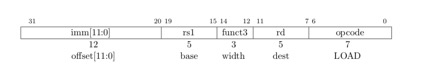
\includegraphics[scale= 1.1]{figures/isa_pgas_format.jpg}
\caption{RISC-V Instruction Format\label{fig:RISC-V ISA Format}}
\end{figure}
 


These registers are and their meaning:

\begin {itemize}
\item PC – Program Counter. This register contains the byte address of the currently executing instruction.
\item Current Domain  (CURRDOM)– This is a 2 bit register.  The value of this register is used to determine the current protection domain.
\item DCAT (DOMCALLTABLE) Domain Call Access Table - used for cross domain calls
\item DCAB (DOMCALLBASE) The base address of the Domain Call Access Table - One per  domain
\item ODTBASE (OBJECTDEFTABLE) –BASE OF Object Definition Table- Object\_ID indexes into table.  Process Wide
\item Object\_ID  base register (CURROBJECT)
\item Current PGAS node id (CURRPGAS).
\item RS1 – the RV128 integer register set.  128 bit wide.
\item HyperPresent – Is this a Hypervisor configured system

\end{itemize}





\pagebreak

In addition to these registers the following memory based operands are used to execute the load instruction.  



\begin{figure}[h]
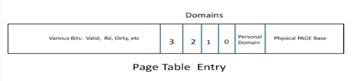
\includegraphics[scale= 1.2]{figures/figure2b_pte.jpg}
\caption{PAGE TABLE ENTRY\label{PAGE TBALE EnTRY}}
\end{figure}
\begin{figure}[h]

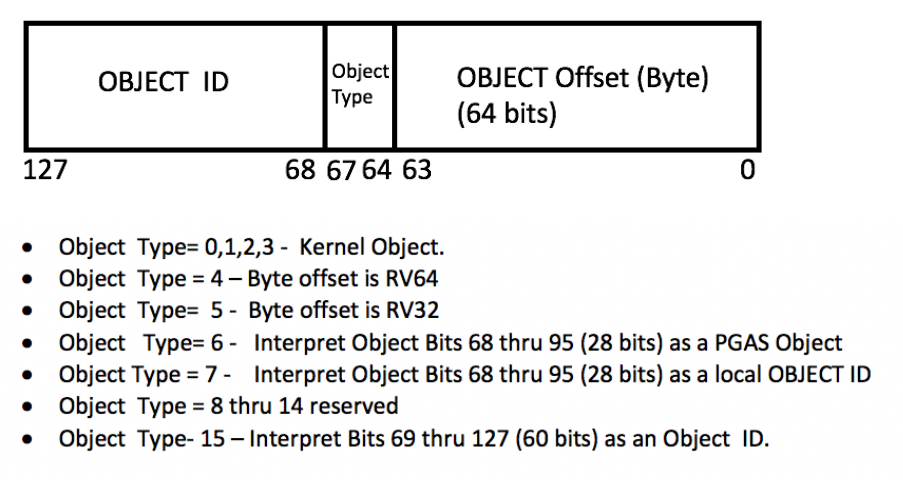
\includegraphics[scale= .5]{figures/pointer_96_bit_object_type_field.jpg}
\begin{center}
\caption{SV128 POINTER FORMAT \label{SV128 POINTER FORMAT}}
\end{center}
\end{figure}

\begin{figure}[h]
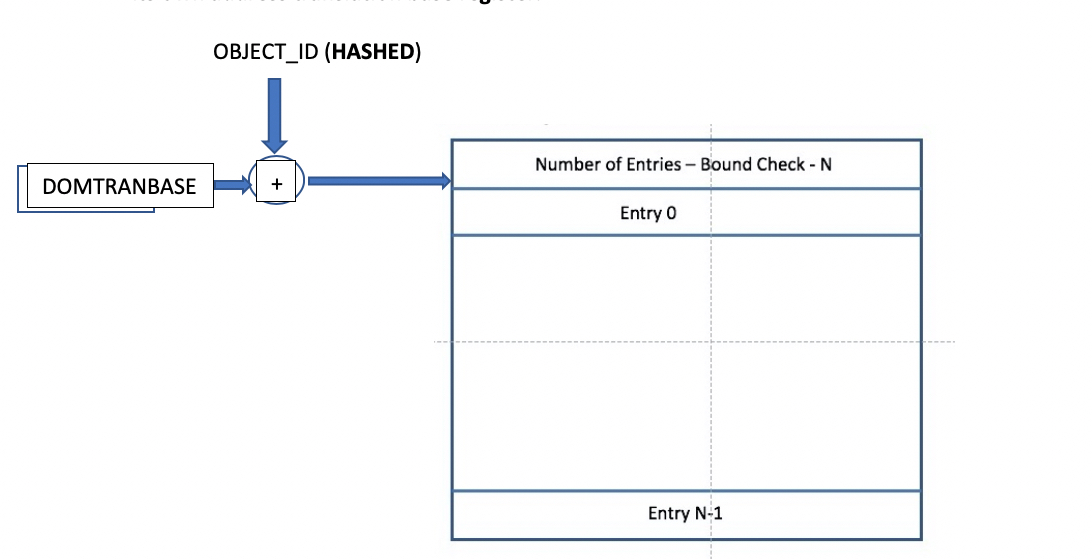
\includegraphics[scale= .3]{figures/figure4a_datt_translation_table.jpg}
\caption{INDEXING INTO OBJECT DEFINITION TABLE} \label{INDEXING INTO OBJECT DEFINITION TABLE}

\end{figure}

 

\pagebreak

\subsection {EXECUTION STEPS}





1)The load instruction is decoded.  


2)The  register  specified by the rs1 field is added to the immediate field to generate a 128 bit address.  This add ONLY uses the lower order 64 bits of these registers.  This is a modular 64 bit add.  The logical address produced has the following format.  The Object\_Id is the value contained in bits [95-64] of register rs1. 


3)Based on the value of the Object\_ID (The object type field -  bits [67-64]) ,  the following happens. If the Object\_ID is  a PGAS node, then do the following:

If the Object\_Id is  equal to the current PGAS node,   then the logical address is locally translated. (see logical to physical translation section)
 
If the Object\_Id is NOT equal to the current PGAS node,  the 128 bit logical address is transmitted to the  designated pgas node.  It is the responsibility of the designated pgas node to local translate this virtual address and respond to the current pgas node with the referenced operand.

If the Object\_Id is NOT a PGAS node.  Then do the following

1.	The Object\_Id is added to the Object Definition Table Base.     As a function of the implementation,  this add may utilize  the hashed value of the Object\_Id.  Before the referenced entry is interpreted,  a bounds check is performed.  The Object\_Id is compared to the first entry in the Object Definition  Table.  If the Object\_Id is greater than the bounds check a fault occurs.  If not the referenced entry is interpreted.

\pagebreak
2.	The valid ODT entry has various control flags.  Among these flags are:
\begin{itemize}
\item the entry valid?
\item Does this entry directly reference an operand, with an explicit bounds check?
\item Does this entry reference a table of Page Table Entries,  and these entries have domain protection bits? 
\end{itemize}









3.	The following happens based on the flags and fields described above
\begin{itemize}

\item If the entry is not valid a fault occurs
\item If the entry is  valid, then
\item If the entry directly references an operand, a  bounds check is performed.  The bounds check value contained within the ODT entry is compared to the byte offset of the 64 bit byte offset of the virtual address.  If the byte offset is less than or equal to the bounds check value, processing continues.  If not a fault occurs.
\item Then the permission  bits in the ODT entry are used to determine if the reference to the operand is valid.  The Current Domain register is used to access the permission bits of the referenced domain the ODT entry.  If the permission is granted,   logical to physical translation occurs,  If the permission is NOT granted,  a fault occurs.
\item If the entry references an operand using  page tables for both permission and logical to  physical translation,  then the following  happens. (not directly referencing an operand)
\item A field in the ODT entry indicates the type of logical to physical entry.  For this description assume that the logical to physical translation specifies RV64. 
\item As part of this specification,  the page size and number of page tables are specified.
\item The 64 bit byte offset is then translated from logical to physical.  During this translation,  the appropriate protection bit in the referenced PTE  is used to determine if the reference is valid.  If not valid,  a protection fault occurs. If valid the physical address derived is used to load the operand from memory to the designated register.
\item The ODT entry can also specify  RV32 and HASHED virtual address logical to physical  translation.

\end{itemize}




It should be noted,  then when a Hypervisor is present,  the register ODT table entry uses for logical to physical   translation is in the Hypervisor address space.  







	






%----------------------------------------------------------------------------------------
%	ACKNOWLEDGEMENTS
%----------------------------------------------------------------------------------------
\newpage
\section*{Acknowledgements}
\label{Acknowledgements}
\addcontentsline{toc}{section}{Acknowledgements}

Many thanks to the following individuals for their advice and 
effort in reviewing this specification: Bruce Jacobs (University 
of Maryland), Kurt Keville (MIT), John Shalf (Lawrence Berkeley 
National Laboratory/NERSC) and Steven Wallach (Micron).

%----------------------------------------------------------------------------------------
%	REFERENCES
%----------------------------------------------------------------------------------------
\newpage
\addcontentsline{toc}{section}{References}
\bibliographystyle{plain}
\bibliography{sv128-arch-spec}

%----------------------------------------------------------------------------------------
%	GLOSSERY
%----------------------------------------------------------------------------------------
%\newpage
%%-- GLOSSARY.TEX

\newglossaryentry{ExtTrans}
{
  name=extended translation,
  description={Extended translation is the process of converting the most
  significant 64 bits, or \textit{extended}, portion of an xBGAS address to
  the respective system architecture's machine descriptor}
}
\newacronym{xBGAS}{xBGAS}{Extended Base Global Address Space}

%\glsaddall
%\glossarystyle{altlist}
%\printglossary[title=List of Terms,toctitle=List of Terms]

\end{appendices}



\end{document}
